\documentclass[11pt,a4paper]{article}

% -----------------------------------------------------------------------------
% Document setup
% -----------------------------------------------------------------------------
\usepackage[T1]{fontenc}
\usepackage[utf8]{inputenc}
\usepackage{lmodern}
\usepackage{microtype}
\usepackage[a4paper,margin=25mm,headheight=14pt]{geometry}

\usepackage{amsmath,amssymb,mathtools}
\usepackage{booktabs}
\usepackage{tabularx}
\usepackage{array}
\usepackage{graphicx}
\usepackage{float}
\usepackage{caption}
\usepackage{subcaption}
\usepackage{xcolor}
\usepackage{enumitem}
\usepackage{listings}
\usepackage{fancyhdr}
\usepackage[hidelinks]{hyperref}

% -----------------------------------------------------------------------------
% Student and assignment details: edit these fields first.
% -----------------------------------------------------------------------------
\newcommand{\studentname}{Rui Luo}
\newcommand{\studentuid}{u8076655}
\newcommand{\coursecode}{COMP8620}
\newcommand{\coursetitle}{Advanced Topics in AI: Intelligent Robotics}
\newcommand{\assignmenttitle}{Assignment 2}
\newcommand{\semester}{Semester 2, 2026}

% -----------------------------------------------------------------------------
% Styling helpers
% -----------------------------------------------------------------------------
\definecolor{anuBlue}{HTML}{1F4E79}
\definecolor{codeBackground}{HTML}{F5F7F9}
\definecolor{codeBorder}{HTML}{D7DCE2}
\definecolor{placeholderGray}{HTML}{606770}

\hypersetup{
  pdftitle={\coursecode\ \assignmenttitle},
  pdfauthor={\studentname\ (\studentuid)},
  colorlinks=true,
  linkcolor=anuBlue,
  citecolor=anuBlue,
  urlcolor=anuBlue
}

\pagestyle{fancy}
\fancyhf{}
\lhead{\coursecode\ -- \assignmenttitle}
\rhead{\studentuid}
\cfoot{\thepage}

\setcounter{secnumdepth}{3}
\setcounter{tocdepth}{2}
\setlist[itemize]{leftmargin=*,itemsep=2pt,topsep=4pt}
\setlist[enumerate]{leftmargin=*,itemsep=2pt,topsep=4pt}
\captionsetup{font=small,labelfont=bf}

\newcommand{\placeholder}[1]{%
  \par\smallskip
  \noindent\textcolor{placeholderGray}{\textit{[Replace this placeholder: #1]}}
  \par\smallskip
}

\newcommand{\finalresult}[1]{%
  \begin{equation}
    \boxed{#1}
  \end{equation}
}

\newcommand{\figureplaceholder}[1]{%
  \begin{center}
    \fcolorbox{codeBorder}{codeBackground}{%
      \parbox[c][45mm][c]{0.86\linewidth}{\centering
        \textcolor{placeholderGray}{\textit{#1}}}}
  \end{center}
}

\lstdefinestyle{python}{
  language=Python,
  basicstyle=\ttfamily\small,
  backgroundcolor=\color{codeBackground},
  frame=single,
  rulecolor=\color{codeBorder},
  numbers=left,
  numberstyle=\scriptsize\color{placeholderGray},
  breaklines=true,
  showstringspaces=false,
  columns=fullflexible,
  keywordstyle=\color{anuBlue}\bfseries,
  commentstyle=\color{placeholderGray}
}

\lstdefinestyle{terminal}{
  basicstyle=\ttfamily\small,
  backgroundcolor=\color{codeBackground},
  frame=single,
  rulecolor=\color{codeBorder},
  breaklines=true,
  showstringspaces=false,
  columns=fullflexible
}

\lstdefinestyle{pseudocode}{
  basicstyle=\ttfamily\small,
  backgroundcolor=\color{codeBackground},
  frame=single,
  rulecolor=\color{codeBorder},
  numbers=left,
  numberstyle=\scriptsize\color{placeholderGray},
  breaklines=true,
  showstringspaces=false,
  columns=fullflexible,
  keywordstyle=\color{anuBlue}\bfseries,
  commentstyle=\color{placeholderGray}\itshape,
  morecomment=[l]{//},
  morekeywords={PROCEDURE,INPUT,OUTPUT,REQUIRE,ENSURE,IF,ELSE,WHILE,FOR,RETURN,FAILURE}
}

\lstdefinestyle{prompt}{
  basicstyle=\ttfamily\small,
  backgroundcolor=\color{codeBackground},
  frame=single,
  rulecolor=\color{codeBorder},
  breaklines=true,
  showstringspaces=false,
  columns=fullflexible
}

\begin{document}
\pagenumbering{gobble}

% -----------------------------------------------------------------------------
% Title page (same layout as A1)
% -----------------------------------------------------------------------------
\begin{titlepage}
  \centering
  \vspace*{30mm}
  {\Large\coursecode\par}
  \vspace{4mm}
  {\Large\coursetitle\par}
  \vspace{16mm}
  {\huge\bfseries\assignmenttitle\ Report\par}
  \vspace{5mm}
  {\large\semester\par}
  \vfill
  \begin{tabular}{@{}ll@{}}
    \toprule
    Student & \studentname \\
    UID & \studentuid \\
    \bottomrule
  \end{tabular}
  \vfill
  {\large The Australian National University\par}
  \vspace{10mm}
\end{titlepage}
\pagenumbering{arabic}

% Replace every placeholder before submission. Prompts must be recorded verbatim.
\section*{Generative AI Disclosure}
\label{sec:ai-disclosure}
OpenAI Codex was used to prepare the report template, review and revise
the Part A answers, implement the first Part B solver and tests, design and run
the first experiments, and draft report text, pseudocode and figures.
Anthropic Claude Code (Claude Opus 5.5) was then used to review the Part B
code and experiments, implement the revised solver (risk-aware guidance and
admissible exploration), redesign and rerun the Part B experiments, analyse
the measured results, and revise the Part B text, tables and figures. The
supplied simulator's transition and reward methods were preserved; their use
and the headless import changes are documented in Part B. Original-language
prompts from all these interactions, including supplied draft answers, are
recorded verbatim in \texttt{AI\_prompts.txt} in the submitted source archive.

% =============================================================================
% Part A: 30 points
% =============================================================================
\section*{Part A: Theory (30 points)}

\subsection*{Question 1: Two-state MDP abstraction (10 points)}
\label{sec:a1}
\begingroup
\setlength{\parindent}{0pt}
\setlength{\parskip}{4pt}
\noindent\textbf{No.}

Let $m=\lceil k/2\rceil$, and define
\[
\phi(s)=
\begin{cases}
L, & 1\le s\le m,\\
R, & m+1\le s\le k.
\end{cases}
\]

An exact MDP abstraction requires a transition function depending only
on the abstract state and action while preserving the original motion
probabilities. In particular, for every action $a$, transition consistency requires
\[
\phi(s_1)=\phi(s_2)
\implies
\sum_{u:\,\phi(u)=R}T(s_1,a,u)
=
\sum_{u:\,\phi(u)=R}T(s_2,a,u).
\]

For $k>4$, consider $s_1=m-1$ and $s_2=m$, both in $L$.
Under $a=\mathrm{moveRight}$,
\[
\begin{aligned}
m-1&\xrightarrow{\,0.7\,}m\in L,
&\qquad m-1&\xrightarrow{\,0.3\,}m-2\in L,\\
m&\xrightarrow{\,0.7\,}m+1\in R,
&\qquad m&\xrightarrow{\,0.3\,}m-1\in L.
\end{aligned}
\]
Hence,
\[
\begin{aligned}
P(R\mid s_1,a)
&=\sum_{u=m+1}^{k}T(m-1,a,u)=0,\\
P(R\mid s_2,a)
&=\sum_{u=m+1}^{k}T(m,a,u)
=T(m,a,m+1)=0.7.
\end{aligned}
\]

Since $0\neq0.7$, transition consistency fails:
no single $T'(L,\mathrm{moveRight},R)$ can represent both states exactly.

Therefore, the proposed abstraction cannot preserve the original motion
uncertainty and is not an exact MDP abstraction.
\par
\endgroup

\clearpage
\subsection*{Question 2: Alpha-vector dominance (10 points)}
\label{sec:a2}
\begingroup
\setlength{\parindent}{0pt}
\setlength{\parskip}{4pt}

Let $p=b(s_1)$. Since $b(s_1)+b(s_2)=1$,
\[
b=(p,1-p),\qquad 0\le p\le1.
\]
For each $\alpha_i\in\Gamma$, let $V_i(p)=\alpha_i\cdot b$. Then
\[
\begin{aligned}
V_1(p)&=10p-5(1-p)=15p-5,\\
V_2(p)&=-5p+10(1-p)=10-15p,\\
V_3(p)&=4p+4(1-p)=4,\\
V_4(p)&=p+2(1-p)=2-p,\\
V_5(p)&=5.5p+(1-p)=1+4.5p.
\end{aligned}
\]

\subsubsection*{(a) Maximal belief intervals (4 points)}

The upper envelope is
\[
V(p)=\max_{\alpha_i\in\Gamma}V_i(p).
\]

\begin{figure}[H]
  \centering
  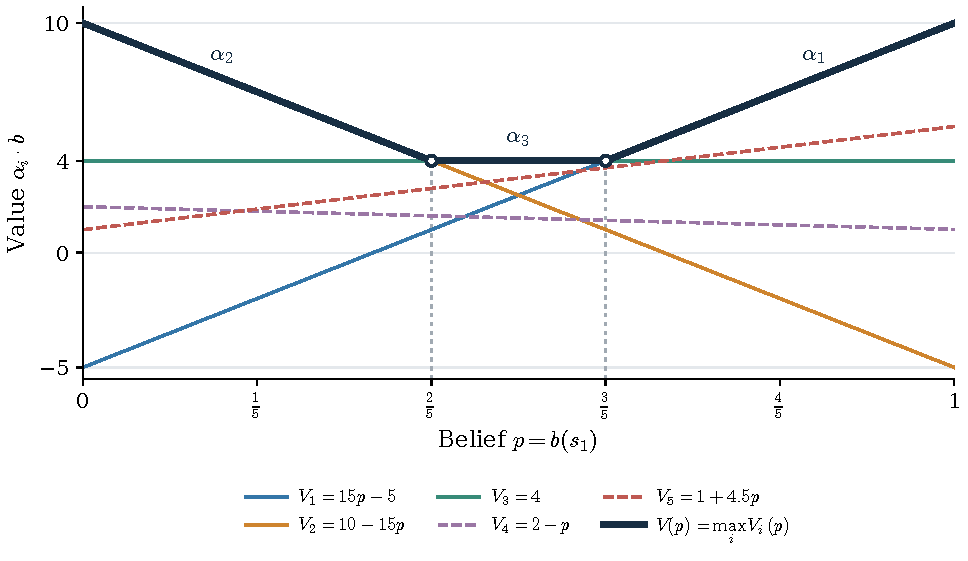
\includegraphics[width=0.96\linewidth]{figures/alpha_envelope.pdf}
\end{figure}

The relevant intersections are
\[
\begin{aligned}
V_2(p)=V_3(p)
&\iff 10-15p=4
\iff p=\frac25,\\
V_1(p)=V_3(p)
&\iff 15p-5=4
\iff p=\frac35.
\end{aligned}
\]

\begin{samepage}
The remaining vectors are never maximal, since
\[
V_4(p)=2-p<4=V_3(p),\qquad 0\le p\le1,
\]
and, using $V_1(p)-V_5(p)=10.5p-6$,
\[
\begin{cases}
V_5(p)\le1+4.5\times\frac35=3.7<4=V_3(p),
    & 0\le p\le\frac35,\\[2pt]
V_1(p)-V_5(p)\ge10.5\times\frac35-6=0.3>0,
    & \frac35\le p\le1.
\end{cases}
\]
\end{samepage}

Since $V_2$ decreases, $V_1$ increases, and $V_3=4$,
\[
V(p)=
\begin{cases}
10-15p, & 0\le p<\frac25,\\
4,      & \frac25\le p\le\frac35,\\
15p-5,  & \frac35<p\le1.
\end{cases}
\]
Therefore, the maximal belief intervals are
\[
\boxed{
\begin{aligned}
\alpha_1 &: \left[\frac35,1\right],\\
\alpha_2 &: \left[0,\frac25\right],\\
\alpha_3 &: \left[\frac25,\frac35\right],\\
\alpha_4,\alpha_5 &: \varnothing.
\end{aligned}
}
\]
At $p=\frac25$, $\alpha_2$ and $\alpha_3$ tie;
at $p=\frac35$, $\alpha_1$ and $\alpha_3$ tie.

\subsubsection*{(b) Pointwise dominance (6 points)}

An $\alpha$-vector can be removed if, at every belief,
another vector has strictly greater value:
\[
\forall b\in B,\quad
\exists\alpha'\in\Gamma:
\alpha\cdot b<\alpha'\cdot b.
\]

For $\alpha_4$,
\[
V_4(p)=2-p<4=V_3(p),\qquad \forall p\in[0,1].
\]
Thus, $\alpha_4$ is strictly dominated by $\alpha_3$.

For $\alpha_5$, the dominating vector may depend on $p$.
From part (a),
\[
\begin{cases}
V_5(p)<V_3(p), & 0\le p\le\frac35,\\
V_5(p)<V_1(p), & \frac35<p\le1.
\end{cases}
\]
These intervals cover $[0,1]$, so $\alpha_5$ also satisfies
the removal condition.

The remaining vectors $\alpha_2$, $\alpha_3$, and $\alpha_1$ are uniquely
maximal at $p=0$, $p=\frac12$, and $p=1$, respectively.
Hence, none satisfies the removal condition.

Therefore,
\[
\boxed{
\Gamma_{\mathrm{remove}}=\{\alpha_4,\alpha_5\},
\qquad
\Gamma_{\mathrm{keep}}=\{\alpha_1,\alpha_2,\alpha_3\}.
}
\]
\par
\endgroup

\clearpage
\subsection*{Question 3: MDP versus POMDP for pedestrian avoidance (10 points)}
\label{sec:a3}
\begingroup
\setlength{\parindent}{0pt}
\setlength{\parskip}{4pt}

Let $c_t,v_t$ be the car's position and speed, and $p_t^i$ the position
of pedestrian $i$. Define
\[
x_t=(c_t,v_t,p_t^1,\ldots,p_t^n).
\]
Positions are observed accurately, and the car measures its own speed.
It chooses an action $a_t$ (accelerate, maintain speed, or brake)
to reach $G$ while avoiding collisions.

\subsubsection*{(a) Scenario suitable for an MDP}

Suppose pedestrians follow known stochastic movement rules: the probabilities
of crossing or continuing along the sidewalk depend only on the current
observable configuration, with no persistent hidden intention.
These memoryless dynamics give
\[
P(x_{t+1}\mid x_{0:t},a_{0:t})
=P(x_{t+1}\mid x_t,a_t).
\]
Thus, $x_t$ is Markov and fully observed, so an MDP with state
$s_t=x_t$ is suitable despite the stochastic pedestrian motion.

\subsubsection*{(b) Scenario suitable for a POMDP}

Now suppose each pedestrian has a persistent but unobservable destination
$g_i$, such as crossing the road or continuing along the sidewalk.
Let $\mathbf g=(g_1,\ldots,g_n)$, and assume motion is Markov conditional
on these destinations. The complete state and observation are
\[
s_t=(x_t,\mathbf g),\qquad o_t=x_t.
\]
At the same observed configuration, two possible joint destinations
can yield different motion distributions:
\[
P(x_{t+1}\mid x_t,a_t,\mathbf g^{(1)})
\neq
P(x_{t+1}\mid x_t,a_t,\mathbf g^{(2)}).
\]
Different motion histories can produce the same $x_t$ but different
beliefs about $\mathbf g$. Hence, $x_t$ alone need not be Markov.
The car maintains
\[
b_t(\mathbf g)=P(\mathbf g\mid x_{0:t},a_{0:t-1})
\]
and predicts motion using
\[
P(x_{t+1}\mid x_t,b_t,a_t)
=\sum_{\mathbf g}
P(x_{t+1}\mid x_t,a_t,\mathbf g)\,b_t(\mathbf g).
\]
The belief is updated as new movements are observed. A POMDP is suitable
because it uses both the observed configuration and the belief over hidden
destinations to select driving actions.
\par
\endgroup

\clearpage
% =============================================================================
% Part B: 35 points
% =============================================================================
\providecommand{\val}[1]{\ifcsname num@#1\endcsname\csname num@#1\endcsname\else\textbf{??#1??}\fi}
\expandafter\def\csname num@BaseMultiDL\endcsname{-2.4}
\expandafter\def\csname num@BaseMultiDLci\endcsname{[-3.7, -0.9]}
\expandafter\def\csname num@BaseMultiDP\endcsname{+3.3}
\expandafter\def\csname num@BaseMultiDPci\endcsname{[+0.4, +6.1]}
\expandafter\def\csname num@BaseMultiFull\endcsname{221}
\expandafter\def\csname num@BaseMultiGreedy\endcsname{229}
\expandafter\def\csname num@BaseMultiLost\endcsname{13}
\expandafter\def\csname num@BaseMultiPairs\endcsname{240}
\expandafter\def\csname num@BaseMultiRescued\endcsname{5}
\expandafter\def\csname num@BaseSingleDL\endcsname{-0.9}
\expandafter\def\csname num@BaseSingleDLci\endcsname{[-1.8, -0.2]}
\expandafter\def\csname num@BaseSingleDP\endcsname{+1.1}
\expandafter\def\csname num@BaseSingleDPci\endcsname{[+0.0, +2.7]}
\expandafter\def\csname num@BaseSingleFull\endcsname{156}
\expandafter\def\csname num@BaseSingleGreedy\endcsname{158}
\expandafter\def\csname num@BaseSingleLost\endcsname{2}
\expandafter\def\csname num@BaseSinglePairs\endcsname{180}
\expandafter\def\csname num@BaseSingleRescued\endcsname{0}
\expandafter\def\csname num@Branch\endcsname{-0.3}
\expandafter\def\csname num@Branchci\endcsname{[-7.5, +6.9]}
\expandafter\def\csname num@BudgetDemoFour3D1024\endcsname{20/20}
\expandafter\def\csname num@BudgetDemoFour3D1024Depth\endcsname{2.9}
\expandafter\def\csname num@BudgetDemoFour3D1024Kept\endcsname{0.63}
\expandafter\def\csname num@BudgetDemoFour3D1024L\endcsname{12.8}
\expandafter\def\csname num@BudgetDemoFour3D16\endcsname{20/20}
\expandafter\def\csname num@BudgetDemoFour3D16Depth\endcsname{2.1}
\expandafter\def\csname num@BudgetDemoFour3D16Kept\endcsname{0.76}
\expandafter\def\csname num@BudgetDemoFour3D16L\endcsname{12.7}
\expandafter\def\csname num@BudgetDemoFour3D2000\endcsname{20/20}
\expandafter\def\csname num@BudgetDemoFour3D2000Depth\endcsname{3.0}
\expandafter\def\csname num@BudgetDemoFour3D2000Kept\endcsname{0.57}
\expandafter\def\csname num@BudgetDemoFour3D2000L\endcsname{12.4}
\expandafter\def\csname num@BudgetDemoFour3D256\endcsname{19/20}
\expandafter\def\csname num@BudgetDemoFour3D256Depth\endcsname{2.7}
\expandafter\def\csname num@BudgetDemoFour3D256Kept\endcsname{0.74}
\expandafter\def\csname num@BudgetDemoFour3D256L\endcsname{15.8}
\expandafter\def\csname num@BudgetDemoFour3D64\endcsname{20/20}
\expandafter\def\csname num@BudgetDemoFour3D64Depth\endcsname{2.5}
\expandafter\def\csname num@BudgetDemoFour3D64Kept\endcsname{0.77}
\expandafter\def\csname num@BudgetDemoFour3D64L\endcsname{12.5}
\expandafter\def\csname num@BudgetDemoOpen2D1024\endcsname{20/20}
\expandafter\def\csname num@BudgetDemoOpen2D1024Depth\endcsname{4.1}
\expandafter\def\csname num@BudgetDemoOpen2D1024Kept\endcsname{0.88}
\expandafter\def\csname num@BudgetDemoOpen2D1024L\endcsname{11.3}
\expandafter\def\csname num@BudgetDemoOpen2D16\endcsname{20/20}
\expandafter\def\csname num@BudgetDemoOpen2D16Depth\endcsname{2.5}
\expandafter\def\csname num@BudgetDemoOpen2D16Kept\endcsname{0.90}
\expandafter\def\csname num@BudgetDemoOpen2D16L\endcsname{11.4}
\expandafter\def\csname num@BudgetDemoOpen2D2000\endcsname{20/20}
\expandafter\def\csname num@BudgetDemoOpen2D2000Depth\endcsname{4.4}
\expandafter\def\csname num@BudgetDemoOpen2D2000Kept\endcsname{0.85}
\expandafter\def\csname num@BudgetDemoOpen2D2000L\endcsname{11.4}
\expandafter\def\csname num@BudgetDemoOpen2D256\endcsname{20/20}
\expandafter\def\csname num@BudgetDemoOpen2D256Depth\endcsname{3.5}
\expandafter\def\csname num@BudgetDemoOpen2D256Kept\endcsname{0.80}
\expandafter\def\csname num@BudgetDemoOpen2D256L\endcsname{11.4}
\expandafter\def\csname num@BudgetDemoOpen2D64\endcsname{20/20}
\expandafter\def\csname num@BudgetDemoOpen2D64Depth\endcsname{3.1}
\expandafter\def\csname num@BudgetDemoOpen2D64Kept\endcsname{0.77}
\expandafter\def\csname num@BudgetDemoOpen2D64L\endcsname{11.3}
\expandafter\def\csname num@BudgetFactorS10A26C51024\endcsname{19/20}
\expandafter\def\csname num@BudgetFactorS10A26C51024Depth\endcsname{3.1}
\expandafter\def\csname num@BudgetFactorS10A26C51024Kept\endcsname{0.65}
\expandafter\def\csname num@BudgetFactorS10A26C51024L\endcsname{15.4}
\expandafter\def\csname num@BudgetFactorS10A26C516\endcsname{18/20}
\expandafter\def\csname num@BudgetFactorS10A26C516Depth\endcsname{2.2}
\expandafter\def\csname num@BudgetFactorS10A26C516Kept\endcsname{0.82}
\expandafter\def\csname num@BudgetFactorS10A26C516L\endcsname{18.2}
\expandafter\def\csname num@BudgetFactorS10A26C52000\endcsname{19/20}
\expandafter\def\csname num@BudgetFactorS10A26C52000Depth\endcsname{3.2}
\expandafter\def\csname num@BudgetFactorS10A26C52000Kept\endcsname{0.61}
\expandafter\def\csname num@BudgetFactorS10A26C52000L\endcsname{16.0}
\expandafter\def\csname num@BudgetFactorS10A26C5256\endcsname{20/20}
\expandafter\def\csname num@BudgetFactorS10A26C5256Depth\endcsname{2.8}
\expandafter\def\csname num@BudgetFactorS10A26C5256Kept\endcsname{0.71}
\expandafter\def\csname num@BudgetFactorS10A26C5256L\endcsname{13.1}
\expandafter\def\csname num@BudgetFactorS10A26C564\endcsname{18/20}
\expandafter\def\csname num@BudgetFactorS10A26C564Depth\endcsname{2.6}
\expandafter\def\csname num@BudgetFactorS10A26C564Kept\endcsname{0.73}
\expandafter\def\csname num@BudgetFactorS10A26C564L\endcsname{17.8}
\expandafter\def\csname num@BudgetStrongWind1024\endcsname{20/20}
\expandafter\def\csname num@BudgetStrongWind1024Depth\endcsname{2.3}
\expandafter\def\csname num@BudgetStrongWind1024Kept\endcsname{0.71}
\expandafter\def\csname num@BudgetStrongWind1024L\endcsname{18.1}
\expandafter\def\csname num@BudgetStrongWind16\endcsname{20/20}
\expandafter\def\csname num@BudgetStrongWind16Depth\endcsname{1.7}
\expandafter\def\csname num@BudgetStrongWind16Kept\endcsname{0.84}
\expandafter\def\csname num@BudgetStrongWind16L\endcsname{16.2}
\expandafter\def\csname num@BudgetStrongWind2000\endcsname{18/20}
\expandafter\def\csname num@BudgetStrongWind2000Depth\endcsname{2.4}
\expandafter\def\csname num@BudgetStrongWind2000Kept\endcsname{0.76}
\expandafter\def\csname num@BudgetStrongWind2000L\endcsname{23.9}
\expandafter\def\csname num@BudgetStrongWind256\endcsname{19/20}
\expandafter\def\csname num@BudgetStrongWind256Depth\endcsname{2.0}
\expandafter\def\csname num@BudgetStrongWind256Kept\endcsname{0.78}
\expandafter\def\csname num@BudgetStrongWind256L\endcsname{21.0}
\expandafter\def\csname num@BudgetStrongWind64\endcsname{19/20}
\expandafter\def\csname num@BudgetStrongWind64Depth\endcsname{1.8}
\expandafter\def\csname num@BudgetStrongWind64Kept\endcsname{0.79}
\expandafter\def\csname num@BudgetStrongWind64L\endcsname{20.6}
\expandafter\def\csname num@CallsC0\endcsname{15,878}
\expandafter\def\csname num@CallsC5\endcsname{16,774}
\expandafter\def\csname num@CeilCorridor\endcsname{63.1}
\expandafter\def\csname num@CeilCorridorSim\endcsname{60.7}
\expandafter\def\csname num@CeilFourSingle\endcsname{94}
\expandafter\def\csname num@CeilFourUncoord\endcsname{16}
\expandafter\def\csname num@CeilFourUncoordCI\endcsname{[13.8, 18.3]\%}
\expandafter\def\csname num@CeilGap\endcsname{70.5}
\expandafter\def\csname num@CeilGapSim\endcsname{69.1}
\expandafter\def\csname num@ClutterNoisy\endcsname{+4.5}
\expandafter\def\csname num@ClutterNoisyA26\endcsname{+4.2}
\expandafter\def\csname num@ClutterNoisyA26ci\endcsname{[-0.6, +8.9]}
\expandafter\def\csname num@ClutterNoisyA6\endcsname{+4.8}
\expandafter\def\csname num@ClutterNoisyA6ci\endcsname{[+3.8, +5.7]}
\expandafter\def\csname num@ClutterNoisyci\endcsname{[+2.1, +6.8]}
\expandafter\def\csname num@ClutterQuiet\endcsname{+1.0}
\expandafter\def\csname num@ClutterQuietA26\endcsname{+0.2}
\expandafter\def\csname num@ClutterQuietA26ci\endcsname{[-0.1, +0.5]}
\expandafter\def\csname num@ClutterQuietA6\endcsname{+1.8}
\expandafter\def\csname num@ClutterQuietA6ci\endcsname{[+1.2, +2.3]}
\expandafter\def\csname num@ClutterQuietci\endcsname{[+0.7, +1.3]}
\expandafter\def\csname num@CompHeuristic\endcsname{+0.6}
\expandafter\def\csname num@CompHeuristicAhi\endcsname{+2.6}
\expandafter\def\csname num@CompHeuristicAint\endcsname{[+0.6, +7.3]}
\expandafter\def\csname num@CompHeuristicAlo\endcsname{-1.4}
\expandafter\def\csname num@CompHeuristicChi\endcsname{+1.7}
\expandafter\def\csname num@CompHeuristicCint\endcsname{[-1.4, +5.8]}
\expandafter\def\csname num@CompHeuristicClo\endcsname{-0.5}
\expandafter\def\csname num@CompHeuristicP\endcsname{-3.8}
\expandafter\def\csname num@CompHeuristicShi\endcsname{+0.6}
\expandafter\def\csname num@CompHeuristicSint\endcsname{[-2.7, +2.6]}
\expandafter\def\csname num@CompHeuristicSlo\endcsname{+0.6}
\expandafter\def\csname num@CompHeuristicci\endcsname{[-1.3, +2.5]}
\expandafter\def\csname num@CompMaxq\endcsname{+3.7}
\expandafter\def\csname num@CompMaxqAhi\endcsname{+1.0}
\expandafter\def\csname num@CompMaxqAint\endcsname{[-7.8, -3.2]}
\expandafter\def\csname num@CompMaxqAlo\endcsname{+6.5}
\expandafter\def\csname num@CompMaxqChi\endcsname{+6.8}
\expandafter\def\csname num@CompMaxqCint\endcsname{[+3.3, +8.9]}
\expandafter\def\csname num@CompMaxqClo\endcsname{+0.7}
\expandafter\def\csname num@CompMaxqP\endcsname{-3.8}
\expandafter\def\csname num@CompMaxqShi\endcsname{+2.6}
\expandafter\def\csname num@CompMaxqSint\endcsname{[-4.7, +0.3]}
\expandafter\def\csname num@CompMaxqSlo\endcsname{+4.8}
\expandafter\def\csname num@CompMaxqci\endcsname{[+2.4, +5.1]}
\expandafter\def\csname num@CompNoguidance\endcsname{+35.7}
\expandafter\def\csname num@CompNoguidanceAhi\endcsname{+37.5}
\expandafter\def\csname num@CompNoguidanceAint\endcsname{[-2.0, +9.0]}
\expandafter\def\csname num@CompNoguidanceAlo\endcsname{+34.0}
\expandafter\def\csname num@CompNoguidanceChi\endcsname{+42.3}
\expandafter\def\csname num@CompNoguidanceCint\endcsname{[+8.7, +17.5]}
\expandafter\def\csname num@CompNoguidanceClo\endcsname{+29.1}
\expandafter\def\csname num@CompNoguidanceP\endcsname{-50.0}
\expandafter\def\csname num@CompNoguidanceShi\endcsname{+33.8}
\expandafter\def\csname num@CompNoguidanceSint\endcsname{[-8.1, +0.2]}
\expandafter\def\csname num@CompNoguidanceSlo\endcsname{+37.7}
\expandafter\def\csname num@CompNoguidanceci\endcsname{[+33.6, +37.8]}
\expandafter\def\csname num@CompNoleaf\endcsname{+0.5}
\expandafter\def\csname num@CompNoleafAhi\endcsname{+0.9}
\expandafter\def\csname num@CompNoleafAint\endcsname{[-1.5, +3.1]}
\expandafter\def\csname num@CompNoleafAlo\endcsname{+0.1}
\expandafter\def\csname num@CompNoleafChi\endcsname{+1.3}
\expandafter\def\csname num@CompNoleafCint\endcsname{[-1.2, +4.4]}
\expandafter\def\csname num@CompNoleafClo\endcsname{-0.3}
\expandafter\def\csname num@CompNoleafP\endcsname{-1.9}
\expandafter\def\csname num@CompNoleafShi\endcsname{+0.3}
\expandafter\def\csname num@CompNoleafSint\endcsname{[-2.5, +1.6]}
\expandafter\def\csname num@CompNoleafSlo\endcsname{+0.7}
\expandafter\def\csname num@CompNoleafci\endcsname{[-1.0, +2.0]}
\expandafter\def\csname num@CompNorisk\endcsname{+1.8}
\expandafter\def\csname num@CompNoriskAhi\endcsname{+2.3}
\expandafter\def\csname num@CompNoriskAint\endcsname{[-2.1, +4.0]}
\expandafter\def\csname num@CompNoriskAlo\endcsname{+1.3}
\expandafter\def\csname num@CompNoriskChi\endcsname{+3.7}
\expandafter\def\csname num@CompNoriskCint\endcsname{[+0.4, +7.0]}
\expandafter\def\csname num@CompNoriskClo\endcsname{-0.1}
\expandafter\def\csname num@CompNoriskP\endcsname{-4.4}
\expandafter\def\csname num@CompNoriskShi\endcsname{+1.5}
\expandafter\def\csname num@CompNoriskSint\endcsname{[-3.9, +2.6]}
\expandafter\def\csname num@CompNoriskSlo\endcsname{+2.1}
\expandafter\def\csname num@CompNoriskci\endcsname{[+0.1, +3.5]}
\expandafter\def\csname num@CompNowidening\endcsname{+1.0}
\expandafter\def\csname num@CompNowideningAhi\endcsname{+2.4}
\expandafter\def\csname num@CompNowideningAint\endcsname{[-0.2, +5.6]}
\expandafter\def\csname num@CompNowideningAlo\endcsname{-0.3}
\expandafter\def\csname num@CompNowideningChi\endcsname{+2.1}
\expandafter\def\csname num@CompNowideningCint\endcsname{[-0.8, +5.3]}
\expandafter\def\csname num@CompNowideningClo\endcsname{-0.1}
\expandafter\def\csname num@CompNowideningP\endcsname{-2.5}
\expandafter\def\csname num@CompNowideningShi\endcsname{+0.9}
\expandafter\def\csname num@CompNowideningSint\endcsname{[-3.2, +2.8]}
\expandafter\def\csname num@CompNowideningSlo\endcsname{+1.1}
\expandafter\def\csname num@CompNowideningci\endcsname{[-0.5, +2.5]}
\expandafter\def\csname num@CompVisitschoice\endcsname{+3.2}
\expandafter\def\csname num@CompVisitschoiceAhi\endcsname{+0.7}
\expandafter\def\csname num@CompVisitschoiceAint\endcsname{[-7.1, -3.0]}
\expandafter\def\csname num@CompVisitschoiceAlo\endcsname{+5.7}
\expandafter\def\csname num@CompVisitschoiceChi\endcsname{+5.7}
\expandafter\def\csname num@CompVisitschoiceCint\endcsname{[+2.8, +7.4]}
\expandafter\def\csname num@CompVisitschoiceClo\endcsname{+0.7}
\expandafter\def\csname num@CompVisitschoiceP\endcsname{-1.2}
\expandafter\def\csname num@CompVisitschoiceShi\endcsname{+2.6}
\expandafter\def\csname num@CompVisitschoiceSint\endcsname{[-3.3, +0.9]}
\expandafter\def\csname num@CompVisitschoiceSlo\endcsname{+3.8}
\expandafter\def\csname num@CompVisitschoiceci\endcsname{[+2.1, +4.3]}
\expandafter\def\csname num@DemoCapShare\endcsname{99}
\expandafter\def\csname num@DemoCapped\endcsname{73}
\expandafter\def\csname num@DemoDecisions\endcsname{74}
\expandafter\def\csname num@DemoMaxPlan\endcsname{9.21}
\expandafter\def\csname num@DemoMinSims\endcsname{1,815}
\expandafter\def\csname num@DepthAlpha005\endcsname{3.5}
\expandafter\def\csname num@DepthAlpha20\endcsname{2.0}
\expandafter\def\csname num@DepthN1\endcsname{3.1}
\expandafter\def\csname num@DepthN4\endcsname{2.5}
\expandafter\def\csname num@DevEpisodes\endcsname{2,880}
\expandafter\def\csname num@DevSettings\endcsname{18}
\expandafter\def\csname num@EffAL\endcsname{-3.8}
\expandafter\def\csname num@EffALci\endcsname{[-5.8, -1.9]}
\expandafter\def\csname num@EffAP\endcsname{-1.1}
\expandafter\def\csname num@EffAPci\endcsname{[-5.2, +3.0]}
\expandafter\def\csname num@EffCL\endcsname{+3.7}
\expandafter\def\csname num@EffCLci\endcsname{[+2.5, +4.9]}
\expandafter\def\csname num@EffCP\endcsname{-2.2}
\expandafter\def\csname num@EffCPci\endcsname{[-4.9, +0.5]}
\expandafter\def\csname num@EffSL\endcsname{+0.5}
\expandafter\def\csname num@EffSLci\endcsname{[-0.9, +1.9]}
\expandafter\def\csname num@EffSP\endcsname{-1.1}
\expandafter\def\csname num@EffSPci\endcsname{[-4.0, +1.8]}
\expandafter\def\csname num@FactCollisions\endcsname{13}
\expandafter\def\csname num@FactObstacle\endcsname{12}
\expandafter\def\csname num@FactSuccess\endcsname{97.6}
\expandafter\def\csname num@FactTimeouts\endcsname{0}
\expandafter\def\csname num@FactVehicle\endcsname{1}
\expandafter\def\csname num@GuideA\endcsname{1539}
\expandafter\def\csname num@GuideB\endcsname{1540}
\expandafter\def\csname num@GuideDL\endcsname{-0.8}
\expandafter\def\csname num@GuideDLci\endcsname{[-1.4, -0.3]}
\expandafter\def\csname num@GuideDP\endcsname{+0.1}
\expandafter\def\csname num@GuideDPci\endcsname{[-0.9, +1.1]}
\expandafter\def\csname num@GuideDuplicates\endcsname{80}
\expandafter\def\csname num@GuideLosses\endcsname{43}
\expandafter\def\csname num@GuidePairs\endcsname{1,680}
\expandafter\def\csname num@GuideWins\endcsname{44}
\expandafter\def\csname num@IntAC\endcsname{-3.6}
\expandafter\def\csname num@IntACci\endcsname{[-4.5, -2.7]}
\expandafter\def\csname num@IntSA\endcsname{-5.0}
\expandafter\def\csname num@IntSAci\endcsname{[-8.3, -1.7]}
\expandafter\def\csname num@IntSC\endcsname{+0.7}
\expandafter\def\csname num@IntSCci\endcsname{[-2.0, +3.5]}
\expandafter\def\csname num@PairAS\endcsname{-4.3}
\expandafter\def\csname num@PairASci\endcsname{[-7.4, -1.3]}
\expandafter\def\csname num@PairCA\endcsname{+7.6}
\expandafter\def\csname num@PairCAci\endcsname{[+5.3, +9.8]}
\expandafter\def\csname num@PairCS\endcsname{+3.2}
\expandafter\def\csname num@PairCSci\endcsname{[+1.7, +4.7]}
\expandafter\def\csname num@ProbeBase\endcsname{69/80}
\expandafter\def\csname num@ProbeBaseGapSteps\endcsname{26}
\expandafter\def\csname num@ProbeRisk\endcsname{65/80}
\expandafter\def\csname num@ProbeRiskGapSteps\endcsname{19}
\expandafter\def\csname num@RandAlpha005\endcsname{40/40}
\expandafter\def\csname num@RandAlpha025\endcsname{38/40}
\expandafter\def\csname num@RandAlpha10\endcsname{36/40}
\expandafter\def\csname num@RandAlpha20\endcsname{30/40}
\expandafter\def\csname num@RandLowNoise\endcsname{78/80}
\expandafter\def\csname num@RandN1\endcsname{38/40}
\expandafter\def\csname num@RandN2\endcsname{36/40}
\expandafter\def\csname num@RandN3\endcsname{38/40}
\expandafter\def\csname num@RandN4\endcsname{32/40}
\expandafter\def\csname num@RandNFourHigh\endcsname{6/10}
\expandafter\def\csname num@RandNFourLow\endcsname{20/20}
\expandafter\def\csname num@RandObstacle\endcsname{9}
\expandafter\def\csname num@RandOverall\endcsname{144/160}
\expandafter\def\csname num@RandTimeouts\endcsname{0}
\expandafter\def\csname num@RandVehicle\endcsname{7}
\expandafter\def\csname num@RegAltitudeDetour\endcsname{20/20}
\expandafter\def\csname num@RegDemoFour3D\endcsname{20/20}
\expandafter\def\csname num@RegDemoOpen2D\endcsname{20/20}
\expandafter\def\csname num@RegNarrowPassage\endcsname{15/20}
\expandafter\def\csname num@RegStrongWind\endcsname{18/20}
\expandafter\def\csname num@RootA26\endcsname{22.4}
\expandafter\def\csname num@RootA6\endcsname{19.1}
\expandafter\def\csname num@RootC0\endcsname{21.8}
\expandafter\def\csname num@RootC5\endcsname{20.7}
\expandafter\def\csname num@SameSTen\endcsname{102}
\expandafter\def\csname num@SameSTotal\endcsname{180}
\expandafter\def\csname num@SetupS20\endcsname{381}
\expandafter\def\csname num@SetupS5\endcsname{95}
\expandafter\def\csname num@SuppFull\endcsname{127/140}
\expandafter\def\csname num@SuppGapRoute\endcsname{11}
\expandafter\def\csname num@SuppGapSteps\endcsname{20}
\expandafter\def\csname num@SuppGapStepsA\endcsname{39}
\expandafter\def\csname num@SuppGreedy\endcsname{125/140}
\expandafter\def\csname num@SuppSuppLayersCross2D\endcsname{20/20}
\expandafter\def\csname num@SuppSuppLayersFour2D\endcsname{20/20}
\expandafter\def\csname num@SuppSuppSingleClutter2D\endcsname{20/20}
\expandafter\def\csname num@SuppSuppSingleExample2D\endcsname{20/20}
\expandafter\def\csname num@SuppSuppSingleSlalom2D\endcsname{20/20}
\expandafter\def\csname num@SuppSuppSingleWallgap2D\endcsname{14/20}
\expandafter\def\csname num@SuppSuppYieldCorridor\endcsname{13/20}
\expandafter\def\csname num@SuppTimeouts\endcsname{0}
\expandafter\def\csname num@TopA26\endcsname{5.8}
\expandafter\def\csname num@TopA6\endcsname{10.7}
\expandafter\def\csname num@TopN1\endcsname{9.0}
\expandafter\def\csname num@TopN4\endcsname{7.2}
\expandafter\def\csname num@TotalEpisodes\endcsname{3,460}
\expandafter\def\csname num@TuneAnchorZ1\endcsname{133/160}
\expandafter\def\csname num@TuneAnchorZ1Eps0\endcsname{133/160}
\expandafter\def\csname num@TuneAnchorZ1W05\endcsname{140/160}
\expandafter\def\csname num@TuneAnchorZ2\endcsname{136/160}
\expandafter\def\csname num@TuneDijkstra\endcsname{140/160}
\expandafter\def\csname num@TuneDijkstraMaxq\endcsname{130/160}
\expandafter\def\csname num@TuneGreedyDijkstra\endcsname{138/160}
\expandafter\def\csname num@TuneGreedyRisk0\endcsname{121/160}
\expandafter\def\csname num@TuneGreedyRisk1\endcsname{138/160}
\expandafter\def\csname num@TuneGreedyVi\endcsname{142/160}
\expandafter\def\csname num@TuneRisk0\endcsname{125/160}
\expandafter\def\csname num@TuneRisk03\endcsname{130/160}
\expandafter\def\csname num@TuneRisk1\endcsname{129/160}
\expandafter\def\csname num@TuneRisk1C01\endcsname{129/160}
\expandafter\def\csname num@TuneRisk1C1\endcsname{123/160}
\expandafter\def\csname num@TuneRisk3\endcsname{126/160}
\expandafter\def\csname num@TuneVi\endcsname{143/160}
\expandafter\def\csname num@TuneViMaxq\endcsname{137/160}

\newcommand{\FactorialRows}{%
5 & 36 & 0 & 20/20 & 13.3 $\pm$ 0.9 & 134.1 $\pm$ 3.9 & 18,413 \\
5 & 36 & 2 & 19/20 & 21.8 $\pm$ 4.6 & 99.0 $\pm$ 23.0 & 19,010 \\
5 & 36 & 5 & 18/20 & 23.4 $\pm$ 6.1 & 89.1 $\pm$ 30.9 & 18,539 \\
5 & 324 & 0 & 20/20 & 12.1 $\pm$ 0.6 & 140.0 $\pm$ 2.1 & 14,951 \\
5 & 324 & 2 & 19/20 & 15.8 $\pm$ 4.9 & 117.8 $\pm$ 35.1 & 16,166 \\
5 & 324 & 5 & 18/20 & 18.1 $\pm$ 6.7 & 110.7 $\pm$ 34.1 & 15,664 \\
5 & 676 & 0 & 20/20 & 12.1 $\pm$ 0.7 & 140.0 $\pm$ 2.2 & 14,730 \\
5 & 676 & 2 & 20/20 & 13.2 $\pm$ 0.9 & 135.7 $\pm$ 3.1 & 15,330 \\
5 & 676 & 5 & 19/20 & 16.2 $\pm$ 4.9 & 120.7 $\pm$ 24.7 & 15,284 \\
10 & 36 & 0 & 20/20 & 13.8 $\pm$ 0.7 & 133.0 $\pm$ 2.5 & 18,368 \\
10 & 36 & 2 & 20/20 & 17.9 $\pm$ 1.2 & 116.0 $\pm$ 4.6 & 18,599 \\
10 & 36 & 5 & 19/20 & 28.1 $\pm$ 3.9 & 75.5 $\pm$ 28.1 & 19,998 \\
10 & 324 & 0 & 20/20 & 12.1 $\pm$ 0.6 & 139.8 $\pm$ 2.0 & 14,939 \\
10 & 324 & 2 & 20/20 & 13.2 $\pm$ 0.7 & 135.7 $\pm$ 2.5 & 15,738 \\
10 & 324 & 5 & 20/20 & 15.7 $\pm$ 0.8 & 125.4 $\pm$ 3.1 & 17,113 \\
10 & 676 & 0 & 20/20 & 12.2 $\pm$ 0.6 & 139.5 $\pm$ 2.1 & 14,759 \\
10 & 676 & 2 & 20/20 & 13.0 $\pm$ 0.7 & 136.7 $\pm$ 2.3 & 15,264 \\
10 & 676 & 5 & 19/20 & 16.8 $\pm$ 4.8 & 115.2 $\pm$ 33.6 & 16,457 \\
20 & 36 & 0 & 20/20 & 13.8 $\pm$ 0.7 & 133.0 $\pm$ 2.5 & 18,368 \\
20 & 36 & 2 & 19/20 & 20.0 $\pm$ 4.6 & 104.8 $\pm$ 23.2 & 18,891 \\
20 & 36 & 5 & 20/20 & 25.4 $\pm$ 1.4 & 90.0 $\pm$ 3.5 & 19,787 \\
20 & 324 & 0 & 20/20 & 12.1 $\pm$ 0.6 & 139.8 $\pm$ 2.0 & 14,939 \\
20 & 324 & 2 & 20/20 & 13.1 $\pm$ 0.7 & 135.6 $\pm$ 2.9 & 15,738 \\
20 & 324 & 5 & 19/20 & 17.8 $\pm$ 4.7 & 114.5 $\pm$ 24.0 & 17,184 \\
20 & 676 & 0 & 20/20 & 12.2 $\pm$ 0.6 & 139.5 $\pm$ 2.1 & 14,759 \\
20 & 676 & 2 & 19/20 & 15.4 $\pm$ 5.0 & 119.6 $\pm$ 35.3 & 15,672 \\
20 & 676 & 5 & 19/20 & 16.4 $\pm$ 4.9 & 120.1 $\pm$ 24.6 & 16,513 \\
}

\newcommand{\FactorEffectRows}{%
State size & -2.0 & [-4.4, 0.3] \\
Action size & -10.2 & [-12.5, -8.0] \\
Clutter & 9.5 & [6.4, 12.5] \\
}

\newcommand{\ComponentRows}{%
Uniform proposals/rollouts & +34.4 [+31.5, +37.4] & -50.0 [-56.0, -44.0] & +33.5 / +35.3 & +34.0 / +34.9 & +30.6 / +38.2$^\ast$ \\
Zero leaf value & +0.0 [-1.5, +1.5] & +0.6 [-2.4, +3.6] & -1.2 / +1.2 & -0.1 / +0.1 & -0.1 / +0.2 \\
No progressive widening & +0.1 [-1.4, +1.5] & +0.0 [-3.3, +3.3] & +0.0 / +0.1 & -0.5 / +0.7 & +0.2 / -0.0 \\
Risk-free guidance & -0.1 [-1.4, +1.2] & -1.9 [-4.7, +1.0] & +0.9 / -1.1 & +0.1 / -0.3 & +0.1 / -0.3 \\
Most-visited final action & +3.4 [+1.7, +5.0] & -1.9 [-6.2, +2.5] & +3.7 / +3.0 & +5.2 / +1.6$^\ast$ & +0.4 / +6.3$^\ast$ \\
Guided policy, no search & -0.4 [-1.7, +0.9] & -0.6 [-3.6, +2.4] & -0.6 / -0.3 & -0.9 / +0.1 & -0.1 / -0.7 \\
}

\newcommand{\ComponentRawRows}{%
Full solver & 20/20 & 18/20 & 20/20 & 19/20 & 20/20 & 20/20 & 20/20 & 19/20 \\
Uniform proposals/rollouts & 9/10 & 0/10 & 9/10 & 0/10 & 10/10 & 0/10 & 9/10 & 0/10 \\
Zero leaf value & 20/20 & 20/20 & 20/20 & 18/20 & 20/20 & 20/20 & 20/20 & 19/20 \\
No progressive widening & 20/20 & 19/20 & 20/20 & 18/20 & 20/20 & 20/20 & 20/20 & 19/20 \\
Risk-free guidance & 20/20 & 16/20 & 20/20 & 19/20 & 20/20 & 19/20 & 20/20 & 19/20 \\
Most-visited final action & 20/20 & 19/20 & 20/20 & 18/20 & 20/20 & 19/20 & 20/20 & 17/20 \\
Guided policy, no search & 20/20 & 18/20 & 20/20 & 19/20 & 20/20 & 19/20 & 20/20 & 19/20 \\
}

\newcommand{\BudgetRows}{%
Open 2D (1) & 16 & 20/20 & 11.4 $\pm$ 0.4 & 2.0 & 2.48 \\
Open 2D (1) & 64 & 20/20 & 11.4 $\pm$ 0.4 & 4.0 & 3.07 \\
Open 2D (1) & 256 & 20/20 & 11.4 $\pm$ 0.4 & 7.7 & 3.54 \\
Open 2D (1) & 1,024 & 20/20 & 11.4 $\pm$ 0.4 & 7.7 & 4.10 \\
Open 2D (1) & 2,000 & 20/20 & 11.3 $\pm$ 0.3 & 7.7 & 4.41 \\
Strong wind (1) & 16 & 19/20 & 21.1 $\pm$ 6.8 & 2.0 & 1.53 \\
Strong wind (1) & 64 & 17/20 & 27.9 $\pm$ 10.8 & 4.0 & 1.72 \\
Strong wind (1) & 256 & 18/20 & 25.4 $\pm$ 9.0 & 8.0 & 1.95 \\
Strong wind (1) & 1,024 & 18/20 & 28.0 $\pm$ 8.9 & 15.0 & 2.20 \\
Strong wind (1) & 2,000 & 18/20 & 26.3 $\pm$ 8.9 & 17.3 & 2.35 \\
Four 3D (4) & 16 & 20/20 & 13.1 $\pm$ 0.7 & 2.0 & 1.95 \\
Four 3D (4) & 64 & 19/20 & 16.2 $\pm$ 7.1 & 4.0 & 2.29 \\
Four 3D (4) & 256 & 20/20 & 12.8 $\pm$ 0.7 & 8.0 & 2.48 \\
Four 3D (4) & 1,024 & 20/20 & 12.9 $\pm$ 0.6 & 16.0 & 2.67 \\
Four 3D (4) & 2,000 & 20/20 & 12.8 $\pm$ 0.6 & 22.8 & 2.75 \\
Factorial S10/A26/C5 (2) & 16 & 19/20 & 17.1 $\pm$ 4.8 & 2.0 & 2.10 \\
Factorial S10/A26/C5 (2) & 64 & 18/20 & 19.2 $\pm$ 6.6 & 4.0 & 2.54 \\
Factorial S10/A26/C5 (2) & 256 & 18/20 & 19.4 $\pm$ 6.6 & 8.0 & 2.79 \\
Factorial S10/A26/C5 (2) & 1,024 & 18/20 & 19.1 $\pm$ 6.6 & 15.9 & 3.03 \\
Factorial S10/A26/C5 (2) & 2,000 & 19/20 & 16.8 $\pm$ 4.8 & 22.5 & 3.13 \\
}

\newcommand{\ClutterControlRows}{%
all 26 & 0.25 & 0 & 20/20 & 12.2 $\pm$ 0.6 & 0 & 0 \\
 &  & 2 & 20/20 & 13.0 $\pm$ 0.7 & 0 & 0 \\
 &  & 5 & 19/20 & 16.8 $\pm$ 4.8 & 0 & 1 \\
 & 0.01 & 0 & 20/20 & 11.0 $\pm$ 0.0 & 0 & 0 \\
 &  & 2 & 20/20 & 11.0 $\pm$ 0.0 & 0 & 0 \\
 &  & 5 & 20/20 & 11.2 $\pm$ 0.2 & 0 & 0 \\
axial 6 & 0.25 & 0 & 20/20 & 13.8 $\pm$ 0.7 & 0 & 0 \\
 &  & 2 & 20/20 & 17.9 $\pm$ 1.2 & 0 & 0 \\
 &  & 5 & 19/20 & 28.1 $\pm$ 3.9 & 0 & 1 \\
 & 0.01 & 0 & 20/20 & 11.6 $\pm$ 0.4 & 0 & 0 \\
 &  & 2 & 20/20 & 13.2 $\pm$ 0.3 & 0 & 0 \\
 &  & 5 & 20/20 & 14.4 $\pm$ 0.5 & 0 & 0 \\
}

\newcommand{\BranchControlRows}{%
$\times1$ & 676 & 19/20 & 14.9 $\pm$ 5.0 & 22.3 & 5.7 \\
$\times2$ & 2,704 & 19/20 & 14.7 $\pm$ 5.0 & 23.0 & 5.1 \\
$\times4$ & 10,816 & 19/20 & 14.6 $\pm$ 5.0 & 23.0 & 5.0 \\
}

\newcommand{\RandomRows}{%
Drones $N$ & 1 & 38/40 & [83, 99] & 10.8 $\pm$ 3.7 & 3.15 \\
 & 2 & 36/40 & [77, 96] & 15.6 $\pm$ 5.0 & 2.77 \\
 & 3 & 38/40 & [83, 99] & 14.2 $\pm$ 3.7 & 2.54 \\
 & 4 & 32/40 & [65, 90] & 21.2 $\pm$ 6.5 & 2.48 \\
Noise $\alpha$ & 0.05 & 40/40 & [91, 100] & 7.7 $\pm$ 0.3 & 3.51 \\
 & 0.25 & 38/40 & [83, 99] & 11.0 $\pm$ 3.7 & 3.10 \\
 & 1 & 36/40 & [77, 96] & 16.0 $\pm$ 4.8 & 2.31 \\
 & 2 & 30/40 & [60, 86] & 27.1 $\pm$ 6.4 & 2.02 \\
}

\newcommand{\RegressionRows}{%
\texttt{demo\_open\_2d} & 20/20 & 0 & 11.7 $\pm$ 0.5 & 0.0380 \\
\texttt{demo\_four\_3d} & 19/20 & 1 & 16.3 $\pm$ 7.0 & 0.0378 \\
\texttt{already\_at\_goals} & 20/20 & 0 & 0.0 $\pm$ 0.0 & 0.0000 \\
\texttt{single\_cell\_goal} & 20/20 & 0 & 0.0 $\pm$ 0.0 & 0.0000 \\
\texttt{one\_reached} & 20/20 & 0 & 8.6 $\pm$ 0.5 & 0.0437 \\
\texttt{swap\_2d} & 20/20 & 0 & 5.2 $\pm$ 0.3 & 0.0379 \\
\texttt{boundary\_reverse} & 20/20 & 0 & 6.0 $\pm$ 0.5 & 0.0377 \\
\texttt{tiny\_2d} & 20/20 & 0 & 1.1 $\pm$ 0.1 & 0.0375 \\
\texttt{thin\_1d} & 20/20 & 0 & 9.8 $\pm$ 1.4 & 0.0374 \\
\texttt{infeasible\_altitude} & 0/20 & 0 & 80.0 $\pm$ 0.0 & 0.0000 \\
\texttt{infeasible\_wall} & 0/20 & 0 & 80.0 $\pm$ 0.0 & 0.0000 \\
\texttt{infeasible\_shared\_goal} & 0/20 & 0 & 80.0 $\pm$ 0.0 & 0.0000 \\
\texttt{horizon\_one} & 0/20 & 0 & 1.0 $\pm$ 0.0 & 0.0489 \\
\texttt{narrow\_passage} & 16/20 & 4 & 27.5 $\pm$ 12.7 & 0.0383 \\
\texttt{altitude\_detour} & 17/20 & 3 & 20.6 $\pm$ 12.0 & 0.0478 \\
\texttt{strong\_wind} & 14/20 & 6 & 39.5 $\pm$ 13.0 & 0.0376 \\
\texttt{three\_3d} & 18/20 & 2 & 17.4 $\pm$ 10.0 & 0.0525 \\
\texttt{four\_2d} & 16/20 & 4 & 24.3 $\pm$ 13.4 & 0.0383 \\
}

\newcommand{\TuningRows}{%
1 & risk0 & 125/160 & 20 & 15 & 24.3 $\pm$ 3.1 & -9.4 [-15.4, -3.3] & +4.5 [+2.1, +7.0] \\
1 & risk0.3 & 130/160 & 19 & 8 & 23.4 $\pm$ 2.9 & -6.2 [-12.2, -0.3] & +3.7 [+1.2, +6.1] \\
1 & risk1 & 129/160 & 20 & 9 & 23.4 $\pm$ 3.0 & -6.9 [-13.4, -0.4] & +3.7 [+0.6, +6.8] \\
1 & risk3 & 126/160 & 23 & 7 & 23.8 $\pm$ 3.0 & -8.8 [-15.5, -2.0] & +4.1 [+1.2, +7.0] \\
1 & risk1\_c0.1 & 129/160 & 21 & 8 & 23.0 $\pm$ 2.9 & -6.9 [-12.2, -1.5] & +3.3 [+1.4, +5.2] \\
1 & risk1\_c1 & 123/160 & 28 & 8 & 25.1 $\pm$ 3.2 & -10.6 [-15.4, -5.9] & +5.4 [+3.3, +7.5] \\
1 & greedy\_risk0 & 121/160 & 17 & 22 & 23.9 $\pm$ 3.2 & -11.9 [-15.8, -8.0] & +4.2 [+2.0, +6.4] \\
1 & greedy\_risk1 & 138/160 & 19 & 4 & 19.8 $\pm$ 2.6 & -1.2 [-5.4, +2.9] & +0.1 [-1.5, +1.6] \\
2 & anchor\_z1 & 133/160 & 19 & 8 & 21.3 $\pm$ 2.8 & -4.4 [-8.6, -0.1] & +1.6 [-0.1, +3.3] \\
2 & anchor\_z2 & 136/160 & 18 & 6 & 20.7 $\pm$ 2.7 & -2.5 [-7.3, +2.3] & +0.9 [-0.6, +2.4] \\
2 & anchor\_z1\_eps0 & 133/160 & 21 & 6 & 21.4 $\pm$ 2.8 & -4.4 [-7.4, -1.4] & +1.7 [+0.6, +2.8] \\
2 & anchor\_z1\_w0.5 & 140/160 & 13 & 9 & 19.7 $\pm$ 2.5 & --- & --- \\
}

\section*{Part B: Multi-drone planning under uncertainty (35 points)}
\begingroup
\setlength{\parindent}{0pt}
\setlength{\parskip}{4pt}

\subsection*{Question 1: MDP formulation (3 points)}
Let $\mathcal G=\{0,\ldots,n_x-1\}\times\{0,\ldots,n_y-1\}
\times\{0,\ldots,n_z-1\}$, with obstacles $O$ and known drone goals $g_i$.
The finite-horizon MDP is $(\mathcal S,\mathcal A,T,R,\gamma)$.

\textbf{States and actions.} A live state is
\[
 s=\bigl((p_i,r_i)_{i=1}^{N},t\bigr),\qquad 0\le t<H,
\]
where $p_i$ is drone $i$'s cell and $r_i$ indicates that it has reached its
goal. Reached drones remain at their goals and occupy those cells.
The state space also contains an absorbing state $\bot$, entered after a
collision, all goals being reached, or the step limit $H$.
Each active drone commands one of $B=26$ neighbour offsets (or $B=8$ with
fixed altitude), giving $\mathcal A=\{0,\ldots,B-1\}^{N}$.
There is no hover action; reached drones ignore their commands.

\textbf{Transitions.} Let $q_i(y_i\mid p_i,r_i,a_i)$ be the supplied,
normalised single-drone target law (Appendix~\ref{app:guidance}).
For a reached drone, $q_i(y_i\mid p_i,1,a_i)=\mathbf1\{y_i=p_i\}$.
Raw targets $y=(y_1,\ldots,y_N)$ are conditionally independent.
Let $F(s,y)$ apply the simulator's position and flag updates and return
$\bot$ on termination. Then
\[
 T(s,a,s')=\sum_{y:F(s,y)=s'}\prod_{i=1}^{N}
 q_i(y_i\mid p_i,r_i,a_i),\qquad T(\bot,a,\bot)=1.
\]
An obstacle hit or shared returned cell terminates the mission; cell swaps
and diagonal crossings are permitted by the supplied collision rule.

\textbf{Reward and objective.} For a sampled outcome $y$, let $K_O$ count
obstacle hits, $K_V$ count drones in shared-cell groups, and $\Delta r_i$
indicate a newly reached goal. The simulator returns
\[
 \widetilde r(s,a,y)=Nc_{\mathrm{step}}+C(K_O+K_V)+G\sum_i\Delta r_i,
 \qquad c_{\mathrm{step}}<0,\ C<0,\ G>0.
\]
Thus $R(s,a)=\mathbb E_y[\widetilde r(s,a,y)\mid s,a]$ and $R(\bot,a)=0$.
The terminal transition receives its reward before absorption. The objective is
\[
 \max_\mu\ \mathbb E_\mu\!\left[
 \sum_{t=0}^{\tau-1}\gamma^t\widetilde r_t\right],
 \qquad \tau=\min\{T_{\mathrm{success}},T_{\mathrm{collision}},H\}.
\]
This encourages fast completion and penalises collisions.

\subsection*{Question 2: Approximate online solver (4 points)}
I use UCT/MCTS with progressive widening~\cite{mdp-lectures,kocsis2006,couetoux2011},
re-planned after every executed step. The supplied generative model samples
outcomes without enumerating the state space or all $26^4=456{,}976$ joint
actions.

\textbf{Guidance.} Cached Dijkstra maps $J_i$ trade path length against
one-step obstacle-slip risk. For a command from $p_i$ towards $q$, the score is
\[
 J_i(q)+0.025\|q-g_i\|_1+\frac{0.3}{\max\{1,d(q)\}}
 +\lambda\ell(p_i)\sum_{\substack{k\ne i\\r_k=0}}
 \sigma(p_k)\mathbf1\{q\in\mathcal N(p_k)\}.
\]
Here $d$ is the supplied obstacle-distance transform;
$\ell$ and $\sigma$ are the normalised intended and per-neighbour slip
probabilities, and $\lambda$ converts collision loss into step-cost units
(Appendix~\ref{app:guidance}). The last term is an inter-drone risk surrogate.
$\mathcal N$ contains physical neighbours at the allowed altitude.
Out-of-grid and obstacle targets receive prohibitive costs; frozen or
already reserved cells receive $10^9$.
\textsc{Greedy} processes drones in index order and minimises this score;
\textsc{Sample} uses random order and samples among the four cheapest
commands within $1.05$ of the minimum, with weights $e^{-3(\mathrm{score}-\min)}$.
\textsc{Explore} samples uniformly from free, in-grid, unreserved targets
when available.

\textbf{The four MCTS components.}
\begin{enumerate}[label=(\arabic*),itemsep=2pt]
\item \textbf{Selection.} Try unvisited admitted actions first; otherwise maximise
\[
 Q(s,a)+c_{\mathrm{UCT}}\sqrt{\frac{\log(N(s)+1)}{N(s,a)}},
 \qquad c_{\mathrm{UCT}}=0.35.
\]
Returns are normalised by $\kappa=\max\{1,N(G+2|C|)\}$.
\item \textbf{Expansion.} The action limit is
$\min\{\lceil0.5\sqrt{N(s)+1}\rceil,\prod_{i:r_i=0}|U_i^{\mathrm{adm}}|\}$.
Admit \textsc{Greedy} first, then \textsc{Explore} with probability $0.15$
and \textsc{Sample} otherwise (at most 12 attempts for a new action).
Each distinct sampled successor has its own child.
\item \textbf{Simulation.} Roll out for at most eight steps, choosing
\textsc{Explore} with probability $0.1$, otherwise \textsc{Greedy}.
Terminal outcomes have zero continuation value; other cutoffs add
\[
 \widehat V(s,h)=Nc_{\mathrm{step}}\sum_{j=0}^{D-1}\gamma^j+
 G\!\!\sum_{\substack{i:r_i=0\\1\le\delta_i\le h}}\gamma^{\delta_i-1},
 \qquad D=\min\{h,\max_{i:r_i=0}\delta_i\}.
\]
$\delta_i$ is the physical breadth-first distance, set to $\infty$ when
unreachable or when frozen goal occupants disconnect the route.
The latter connectivity check is cached on maps of at most 20,000 cells.
Tree depth is capped at eight.
\item \textbf{Backpropagation.} Back up $v=R_{\mathrm{sample}}/\kappa+\gamma v'$;
increment edge and node visits and update the edge mean and sample variance
using Welford's recurrence.
\end{enumerate}

\textbf{Root decision.} Let $a_g$ be the greedy action and $\hat\sigma^2$
the pooled within-action variance. Among visited actions, define
\[
 m(a)=Q(a)-Q(a_g)-z_{\mathrm{sw}}\hat\sigma
 \sqrt{\frac1{N(a)}+\frac1{N(a_g)}},\qquad z_{\mathrm{sw}}=1.
\]
Execute the action with largest positive $m(a)$; otherwise keep $a_g$.
With no completed trial, use $a_g$ directly.
This variance-aware switching heuristic has no formal policy-improvement
guarantee. Parameters were selected on separate
development layouts (Appendix~\ref{app:tuning}).

\noindent\begin{minipage}{\linewidth}
\begin{lstlisting}[style=pseudocode,basicstyle=\ttfamily\footnotesize,caption={Online UCT; rollout and admission rules are defined above.}]
PROCEDURE PLAN(s, budget, K = 2000)
    deadline <- NOW + max(0, 0.97 * min(budget, 10) - 0.002)
    a_g <- GREEDY(s); root <- empty node; h <- H - t; sims <- 0
    WHILE NOW < deadline AND sims < K AND h > 0 AND not all reached:
        TRY: SEARCH(root, s, h, 0); sims += 1
        ON Deadline: BREAK
    RETURN root decision above, or a_g if no trial completed

PROCEDURE SEARCH(node, s, h, depth)
    IF h = 0 OR all reached: RETURN 0
    IF depth >= 8: RETURN ROLLOUT(s, h)
    admit an action under the expansion rule, if permitted
    a <- unvisited action first, otherwise argmax UCB
    (s', r, done) <- SIMULATE(s, a)  // check deadline before call
    IF done: v <- 0
    ELSE IF child(node, a, s') is new:
        create child; v <- ROLLOUT(s', h - 1)
    ELSE: v <- SEARCH(child(node, a, s'), s', h - 1, depth + 1)
    v <- r / kappa + gamma * v
    update visits, mean and variance; RETURN v
\end{lstlisting}
\end{minipage}
\textsc{Rollout} discounts sampled rewards and the terminal/cutoff value
defined above. It may stop at the deadline and return a leaf estimate;
a deadline exception before a simulator call aborts that trial.
The planner tracks the remaining horizon because \texttt{simulate} does
not enforce the execution step limit.

\subsection*{Question 3: Implementation and demonstration (8 points)}
\texttt{run\_u8076655.py} executes the closed-loop planner. The supplied
simulator is vendored at revision \texttt{ea3cbfe}; AST checks verify that its
core dynamics and rewards are unchanged~\cite{provided-code}.
The planner uses \texttt{get\_config()}, \texttt{simulate()} and
\texttt{num\_actions}, with separate planning and execution RNGs.
From the extracted archive's top-level directory:
\begin{lstlisting}[style=terminal]
python -m pip install -r requirements.txt
python run_u8076655.py --config <scenario.yaml>
\end{lstlisting}
Each step prints progress; \texttt{--visualize} enables the optional Vedo
viewer. Planning is serial, with a default 9.5\,s allowance and 2,000-trial
cap. The clock is checked before every simulator call, with a margin for
returning the action. Local validation results follow.
All 45 unit tests pass. Local single-process runs with the
default 9.5-second allowance (seed 0) give:

\begin{table}[H]
\centering\small
\renewcommand{\arraystretch}{1.13}
\begin{tabular*}{\linewidth}{@{\extracolsep{\fill}}llrrrr@{}}
\toprule
Task & Status & Steps & Sims/step & Mean (s) & Max (s) \\
\midrule
Open 2D, 1 drone, 8 actions & success & 14 & 2,000 & 4.53 & 7.42 \\
Supplied example, 2 drones & success & 17 & 2,000 & 5.59 & 7.48 \\
Strong wind, 1 drone, $\alpha=3$ & success & 30 & 2,000 & 4.72 & 6.34 \\
Four 3D, 5 obstacles & success & 13 & 1,986 & 6.27 & 9.21 \\
\bottomrule
\end{tabular*}
\end{table}


\clearpage
\subsection*{Question 4: Experimental investigation (20 points)}
\subsubsection*{Experimental design}
The main evaluation uses 2,000 simulations per decision; S3 includes
ablations and a zero-search policy, and S4 varies the simulation cap.
Experimental runs use a relaxed wall-clock cap to isolate search effort.
The demo instead stops at the first of its time and trial limits, so these
are different budget protocols. Conditions share execution seeds 0--19
unless noted, with comparisons paired within each scenario.
Development layouts were excluded from evaluation. Original run hashes are
retained in the metadata; subsequent planner patches are checked separately
before these results are reused: replaying all $\val{EquivTotal}$ reported
seed-0 episodes with the submitted planner reproduced $\val{EquivIdentical}$
of them step for step (\texttt{results/planner\_equivalence.json}).

\begin{table}[H]
\centering\footnotesize
\begin{tabularx}{\linewidth}{@{}>{\raggedright\arraybackslash}p{1.25cm}
>{\raggedright\arraybackslash}X>{\raggedright\arraybackslash}p{4.7cm}@{}}
\toprule Set & Controlled scenarios & Question and expectation \\
\midrule
S1 (540) &
$3^3$ factorial: $12\times n_y\times3$ grids, $n_y=5,10,20$;
6/18/26 commands per drone ($|A|=36/324/676$); 0/2/5 nested obstacles.
Two drones, $\alpha=0.25$, $H=60$. &
Rank the three factors and test interactions. Off-route cells should have
little effect; richer control may help; clutter adds detours and slip risk. \\
S2 (160) &
S1 clutter layouts at $\alpha=0.01$ with 6/26 commands;
duplicate command labels $\times2,\times4$ without changing physics. &
Separate geometric detours from noise, and control authority from branching. \\
S3 (880) &
Five ablations and the search-free policy at all eight low/high S1 corners.
Uniform proposals use ten seeds; others use twenty. &
Measure how component effects change with each complexity factor. \\
S4 (400) &
16/64/256/1,024/2,000 simulations on open 1-drone, strong-wind 1-drone,
cluttered 2-drone and 3D 4-drone tasks. &
Test whether additional search improves completion as tasks get harder. \\
S5 (160) &
$N=1,2,3,4$ crossed with $\alpha=0.05,0.25,1,2$;
one random $8\times6\times3$ layout per pair, ten seeds each. &
Check performance beyond the factorial and joint growth of state/action spaces. \\
\bottomrule
\end{tabularx}
\caption{Evaluation sets; parentheses give episode counts. A further 360
regression episodes are listed in Appendix~\ref{app:regression}.}
\end{table}

A further 520 search-free runs pair the base policy with the completed
regression and generated suites (Appendix~\ref{app:regression}).

\textbf{Metrics.} With $F$ free cells, there are up to $F^N$ positional
configurations and $B^N$ joint commands.
Success means all goals reached within $H$ without collision.
Penalised completion length is $L=\text{steps}$ on success and $L=H$ on
failure. Success proportions have Wilson 95\% intervals; continuous means
have Student-$t$ intervals $\bar x\pm t_{0.975,n-1}s/\sqrt n$.
High-minus-low factor effects average the other factors within each seed;
component effects pair each ablation with the full solver before averaging
corners. Their 95\% intervals use seed blocks. Full condition means,
returns and search diagnostics are in Appendix~\ref{app:factorial}--\ref{app:layouts}.
Experiments ran serially on macOS 26.6.2 (\texttt{x86\_64}), using
Python 3.12.9, NumPy 1.26.4, SciPy 1.15.1,
and PyYAML 6.0.2. No GPU, multiprocessing or threaded planning
was used. Setup is timed separately from online decisions.


\subsubsection*{S1: effects of the three complexity factors}
\begin{figure}[H]
\centering
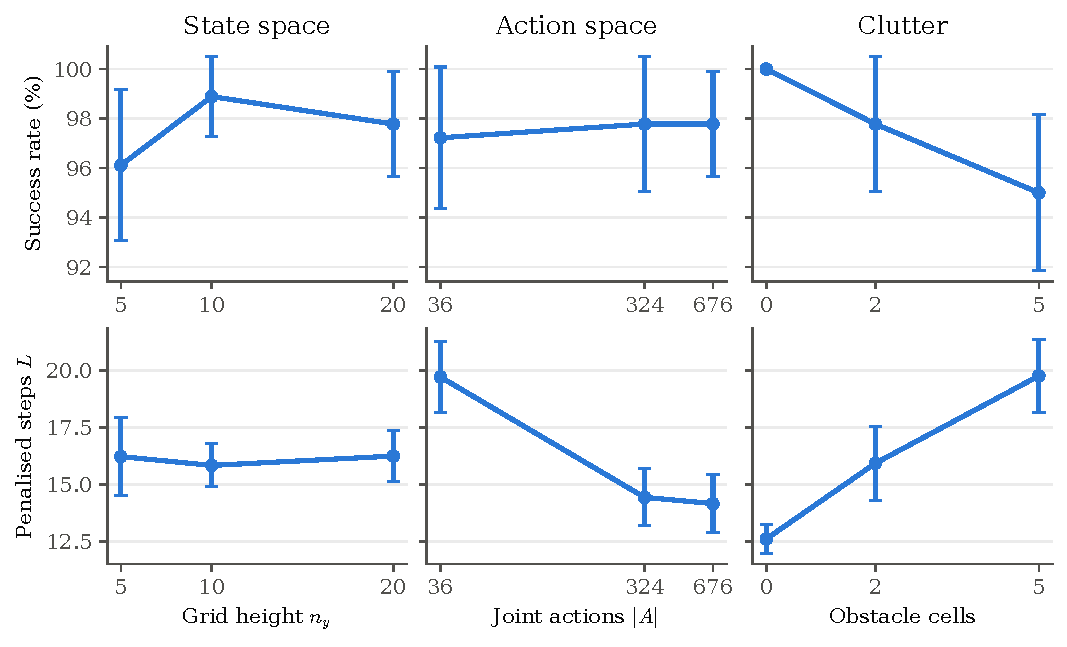
\includegraphics[width=0.95\linewidth]{figures/complexity_effects.pdf}
\caption{Factorial marginal means; bars are 95\% intervals over 20 seed blocks.}
\end{figure}
\begin{table}[H]
\centering\small
\begin{tabular}{@{}lll@{}}
\toprule Factor (high minus low) & $\Delta L$ (95\% CI) & $\Delta$success (pp; 95\% CI) \\
\midrule
\FactorEffectRows
\bottomrule
\end{tabular}
\end{table}

\textbf{Clutter causes the largest degradation within these tested levels.}
Adding five obstacles raises $L$ by $\val{EffCL}$ steps $\val{EffCLci}$ and
changes success by $\val{EffCP}$ percentage points $\val{EffCPci}$.
The solver succeeds in $\val{FactSuccess}\%$ of S1 episodes; all
$\val{FactCollisions}$ failures are collisions and none reaches the horizon.

\textbf{State-space padding has little observed effect.}
For $n_y=10$ versus 20, $\val{SameSTen}$ of $\val{SameSTotal}$ paired
episodes are identical. The extra off-route cells do not affect these runs;
this tests padding, not the effect of longer routes or additional drones.
Mean map setup grows from $\val{SetupS5}$ to $\val{SetupS20}$\,ms
($n_y=5$ versus 20), outside per-decision planning.

\textbf{Richer commands shorten routes.}
Changing 6 to 26 directions gives $\Delta L=\val{EffAL}$ $\val{EffALci}$;
the success difference is not statistically resolved.
The action--clutter interaction is $\val{IntAC}$ $\val{IntACci}$ steps,
consistent with diagonal/vertical moves easing obstacle
avoidance. Neither state-related interaction is resolved
($S\times C$: $\val{IntSCci}$; $S\times A$: $\val{IntSAci}$).

\subsubsection*{S2: geometry, noise and action branching}
At $n_y=10$, the clutter effect averaged over the two command sets is
$\val{ClutterNoisy}$ steps $\val{ClutterNoisyci}$ at $\alpha=0.25$,
versus $\val{ClutterQuiet}$ $\val{ClutterQuietci}$ at $\alpha=0.01$,
where all episodes succeed. Thus geometry still adds detour cost, while
noise substantially increases the observed clutter penalty.
The supplied transition law raises slip probability near obstacles;
its no-obstacle distance-transform convention is noted in
Appendix~\ref{app:guidance}.

Duplicating command labels up to $|A|=10{,}816$ changes $L$ by only
$\val{Branch}$ $\val{Branchci}$ and leaves the admitted root-action count
near 23. This separates pure label branching from the extra control
authority in S1. Detailed controls, including the visit share of the
\emph{executed} action, appear in Appendix~\ref{app:controls}.

\subsubsection*{S3: component effects as complexity increases}
\begin{figure}[!htbp]
\centering
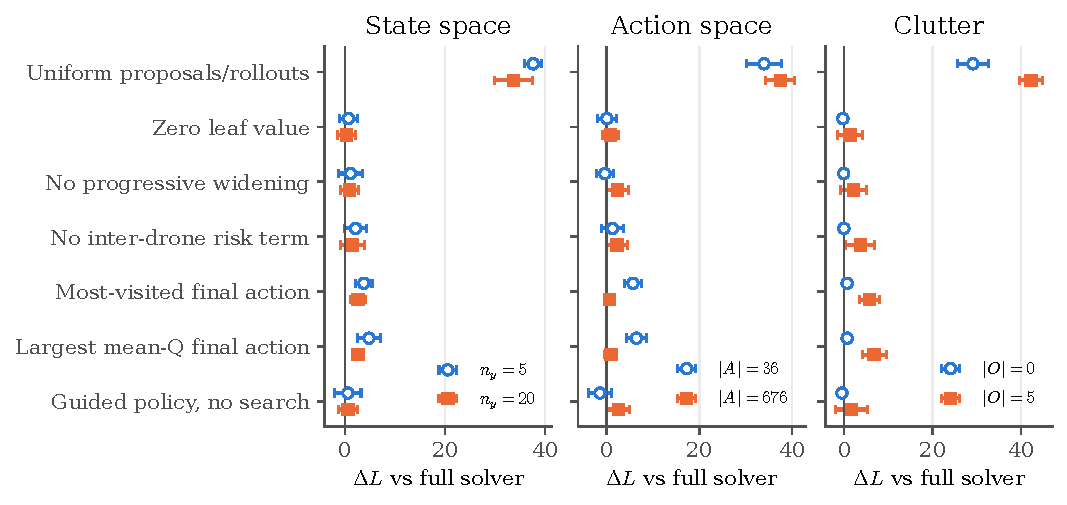
\includegraphics[width=\linewidth]{figures/component_effects.pdf}
\caption{Paired change in $L$ after removing a component at low/high factor
levels (open/filled markers); 95\% seed-block intervals.
Positive values favour the full solver.}
\end{figure}

\textbf{Guidance in expansion and rollout} has the largest measured effect.
Uniform proposals/rollouts raise $L$ by $\val{CompNoguidance}$
$\val{CompNoguidanceci}$ and change success by $\val{CompNoguidanceP}$\,pp.
The loss grows from $\val{CompNoguidanceClo}$ without obstacles to
$\val{CompNoguidanceChi}$ with five; the clutter interaction excludes zero
($\val{CompNoguidanceCint}$), whereas its state/action interactions do not.
This ablation removes both route guidance and admissible-target filtering.

\textbf{Root choice} also matters: most-visited selection raises $L$ by
$\val{CompVisitschoice}$ $\val{CompVisitschoiceci}$, and executing the
largest-mean-$Q$ action raises it by $\val{CompMaxq}$ $\val{CompMaxqci}$.
Both increases are larger with clutter (interaction intervals
$\val{CompVisitschoiceCint}$ and $\val{CompMaxqCint}$) and smaller with richer
commands ($\val{CompVisitschoiceAint}$ and $\val{CompMaxqAint}$). These
comparisons support the chosen switching rule on these tasks; they do not
make its estimated margin a calibrated confidence bound.

\textbf{Widening and the leaf value} have no statistically resolved effects
across these corners ($\val{CompNowidening}$ $\val{CompNowideningci}$ and
$\val{CompNoleaf}$ $\val{CompNoleafci}$; full estimates in
Appendix~\ref{app:components}). Routes are roughly eleven steps, comparable
to the sampled tree depth plus eight-step rollout, which may limit the leaf
value's contribution. \textbf{The inter-drone risk term} does matter:
removing it raises $L$ by $\val{CompNorisk}$ $\val{CompNoriskci}$ and changes
success by $\val{CompNoriskP}$\,pp, mostly with clutter (interaction
$\val{CompNoriskCint}$).

\textbf{Search versus its base policy.}
Removing search changes $L$ by $\val{CompHeuristic}$ $\val{CompHeuristicci}$
overall, but its action interaction is resolved ($\val{CompHeuristicAint}$):
removing search raises $L$ with 26 commands ($\val{CompHeuristicAhi}$),
while the change with 6 commands is unresolved ($\val{CompHeuristicAlo}$).
In the regression and generated suites, search rescues
$\val{BaseMultiRescued}$ multi-drone episodes and loses $\val{BaseMultiLost}$
and removing it changes $L$ by $\val{BaseMultiDL}$
$\val{BaseMultiDLci}$ (Appendix~\ref{app:regression}). With value guidance,
search has no consistent completion benefit across the evaluated suites;
the measured performance is largely explained by the guided base policy.


\subsubsection*{S4: search budget}
\begin{figure}[H]
\centering
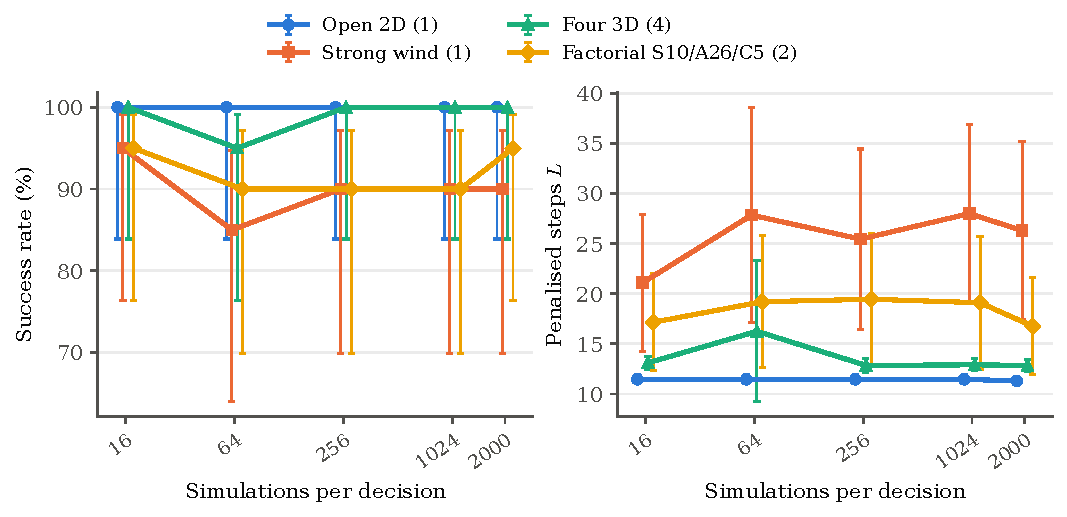
\includegraphics[width=0.95\linewidth]{figures/budget_curve.pdf}
\caption{Success and $L$ versus simulations per decision; 20 runs per point,
with Wilson and $t$ 95\% intervals. Drone counts are in parentheses.}
\end{figure}
There is no consistent improvement from 16 to 2,000 simulations across
these four tasks. In the four-drone case, success is
$\val{BudgetDemoFour3D16}$ and $\val{BudgetDemoFour3D2000}$ respectively,
while mean new-node depth grows from $\val{BudgetDemoFour3D16Depth}$ to
$\val{BudgetDemoFour3D2000Depth}$ and the fraction keeping the base action
falls from $\val{BudgetDemoFour3D16Kept}$ to $\val{BudgetDemoFour3D2000Kept}$.
Search therefore changes decisions without a demonstrated completion
benefit here. Overlapping intervals do not establish budget equivalence.

\subsubsection*{S5: generated layouts}
Across the crossed drone-count/noise set, $\val{RandOverall}$ episodes
succeed. At $\alpha\le0.25$, $\val{RandLowNoise}$ runs succeed,
including $\val{RandNFourLow}$ with four drones; four drones at $\alpha=2$
succeed in $\val{RandNFourHigh}$. This indicates sensitivity to noise in
the tested layouts, while increasing $N$ jointly enlarges state and action
spaces. Mean new-node depth is $\val{DepthN1}$ for one drone and
$\val{DepthN4}$ for four, consistent with less successor reuse when joint
outcomes multiply. Each $(N,\alpha)$ pair has only one layout, so the
per-layout results in Appendix~\ref{app:layouts} do not isolate layout effects.
For the four-drone layout at $\alpha=2$, joint value iteration was not attempted
($140^4\approx4\times10^8$ joint positions per step). Each drone alone could
achieve at least $\val{CeilFourSingle}\%$ success when other drones are removed.
Executing those policies together gives $\val{CeilFourUncoord}\%$ success
(1,000 diagnostic runs; Wilson 95\% interval $\val{CeilFourUncoordCI}$),
compared with $\val{RandNFourHigh}$ for the solver. The different sample sizes
and unpaired comparison do not establish a solver advantage or isolate the
cause of failure. They motivate further coordination tests
(\texttt{results/ceilings.json}).

\subsubsection*{Conclusions and limitations}
Within the factorial's tested levels, clutter causes the largest
degradation; extra control directions help, while off-route state padding
has little observed effect. Guided expansion/rollout and the root decision
rule contribute most, particularly in clutter. Additional search has no
demonstrated completion benefit over the guided base policy on these tasks.

The ranking is specific to two drones, $\alpha=0.25$ and the chosen layouts.
The $t$ intervals for bimodal $L$ are approximate, and generated-layout
replication is limited. Fixed-simulation experiments do not reproduce a
binding demo deadline on every machine. Static guidance does not model
detours around frozen drones beyond the leaf disconnection check; observed
collisions have not been proved unavoidable. The leaf estimate charges no
collision risk, so search can postpone an unavoidable risky passage beyond
its horizon: in the wall-gap case (Figure~\ref{fig:risk-maps}, bottom
right) successful runs averaged
$\val{SuppGapSteps}$ steps for an $\val{SuppGapRoute}$-step route. A
risk-charged leaf shortened those runs in a small probe
($\val{ProbeBaseGapSteps}$ to $\val{ProbeRiskGapSteps}$ steps) without raising
success ($\val{ProbeRisk}$ versus $\val{ProbeBase}$ over eight tasks), so it was
not adopted.
Stronger coordination tasks and outcome widening or open-loop
trees would be useful follow-up tests.

\par
\endgroup


\clearpage
\appendix
\section{Supporting definitions and results}
\label{app:details}
Complete regression, budget and tuning data remain in the source archive.
The six original evaluation suites retain their generating hashes;
all \val{EquivTotal} original seed-0 traces replay identically with the
current planner (\texttt{results/planner\_equivalence.json}).
Baseline and supplementary runs use the current planner directly.
\subsection{Algorithm definitions}
\label{app:guidance}
For a free in-grid target command, let $\mathcal N(q)$ be the physical
neighbours of $q$ and $V(q)=|\mathcal N(q)|$. The supplied motion law gives
\[
 \begin{aligned}
 \pi(q)&=\frac{d(q)}{d(q)+\alpha},&
 M(q)&=\pi(q)+(V(q)-1)\frac{1-\pi(q)}{B-1},\\
 \ell(q)&=\frac{\pi(q)}{M(q)},&
 \sigma(q)&=\frac{1-\pi(q)}{(B-1)M(q)}.
 \end{aligned}
\]
\textbf{Value guidance (submitted).} For command $a$ from free cell $p$, the
intended neighbour has weight $\pi(p)$, every other in-grid neighbour
$(1-\pi(p))/(B-1)$, the row is renormalised, and mass on obstacle cells is a
terminal crash. Value iteration uses these exact rows (stored sparsely) with
$r_i=c_{\mathrm{step}}+C\Pr(\text{crash})+G\Pr(\text{arrival at }g_i)$ and
$V_{i,h}(g_i)=0$, because arrival is terminal for that drone. Per-horizon
action values are kept when $nA(H+1)N\le2.5\times10^7$ ($n$ free cells, $A$
commands) on grids of at most 20,000 cells; otherwise the planner uses the
Dijkstra guidance below. On the demo maps this takes under 0.2\,s before
the first decision.

\textbf{Dijkstra guidance (comparison A).} Entry costs are
$1+\lambda\rho(q)$ for a non-goal cell and 1 for the goal, where
\[
 \rho(q)=|\mathcal N(q)\cap O|\sigma(q),\qquad
 \lambda=\frac{w(G+|C|)}
 {\max\{|c_{\mathrm{step}}|,10^{-3}(G+|C|),10^{-9}\}},\quad w=1.
\]
With $w=0$, these are breadth-first distances. The supplied empty-map
distance transform uses a virtual point beyond the grid corner, so slips
remain possible without obstacles.

Grid boundaries are not obstacles: out-of-grid outcome mass is removed
before normalisation. The simulator encodes a joint command as
\[
 a_{\mathrm{int}}=\sum_{i=1}^{N}a_iB^{i-1}.
\]
Maps are built for at most 150,000 cells. Larger grids use Chebyshev
distance without a risk map; fixed-altitude goals on another layer
remain unreachable. Frozen-goal disconnection checks are cached by
drone and reached subset for at most 20,000 cells. Above that size,
the leaf uses static reachability. These fallbacks are implementation
limits, not guarantees of safe coordination.

A rollout cut off after $L$ sampled steps returns
\[
 \sum_{j=0}^{L-1}\gamma^j r_j/\kappa+
 \gamma^L\widehat V(s_L,h-L)/\kappa,
\]
with zero continuation on termination. For an edge sample $v$, update
\[
 n\gets n+1,\quad \Delta\gets v-Q,\quad
 Q\gets Q+\Delta/n,\quad S\gets S+\Delta(v-Q).
\]
The pooled root variance is $\hat\sigma^2=\sum_a S_a/\sum_a(n_a-1)$ over
visited actions, or zero when the denominator is zero.

\subsection{Development-set parameter selection}
\label{app:tuning}
Sixteen layouts cross $N=1,2,3,4$ with
$\alpha\in\{0.25,0.5,1,2\}$ on $10\times10\times1$ or
$10\times10\times5$ grids, with 0--5 obstacles (generator seed 4620).
Each setting uses ten execution seeds and at most 500 simulations per
decision; search-free settings use none. These $\val{DevEpisodes}$
development episodes are separate from all $\val{TotalEpisodes}$ evaluation
episodes.

Round 1 compares risk weights, UCT constants and search-free policies
under most-visited root choice and widening coefficient 1.5.
Round 2 compares the anchored rule, its threshold and rollout exploration,
and widening coefficient 0.5. The selected setting is
\texttt{anchor\_z1\_w0.5}: risk weight 1, UCT constant 0.35,
switch threshold 1, widening coefficient 0.5 and rollout exploration 0.1.
Here the suffix \texttt{w0.5} denotes widening, not the risk weight.
Round 3 compares that Dijkstra guidance with single-drone value-iteration
guidance, each with the anchored rule and with largest-mean-$Q$ root choice,
plus both search-free policies. The selection criterion required no worse
observed success count or mean $L$. Value guidance met it
($\val{TuneVi}$ versus $\val{TuneDijkstra}$ successes), whereas
largest-mean-$Q$ choice raised $L$ under both guidances
($\val{TuneDijkstraMaxq}$ and $\val{TuneViMaxq}$). The round-3 Dijkstra arm
reproduces the round-2 selected setting exactly.
Development tables retain the planner hashes recorded for those versions;
all evaluation suites were rerun with the final implementation.

\begin{table}[H]
\centering\small
\caption{Development results: 160 episodes per setting. $L$: mean
$\pm$95\% interval half-width. $\Delta L$: paired change from the selected
setting, with a 95\% interval over ten seed blocks; lower is better.
Selection across $\val{DevSettings}$ settings makes these exploratory comparisons
optimistic for the development layouts.}
\begin{tabular*}{\linewidth}{@{\extracolsep{\fill}}rlcrr@{}}
\toprule Round & Setting & Success & $L$ & $\Delta L$ (95\% CI) \\
\midrule
\TuningSummaryRows
\bottomrule
\end{tabular*}
\end{table}

\subsection{Factorial results}
\label{app:factorial}
\begingroup
\small
\newcolumntype{R}[1]{>{\raggedleft\arraybackslash}p{#1}}
\newcolumntype{C}[1]{>{\centering\arraybackslash}p{#1}}
\setlength{\LTleft}{0pt}
\setlength{\LTright}{\fill}
\begin{longtable}{@{}R{.055\linewidth}R{.075\linewidth}R{.055\linewidth}
C{.12\linewidth}R{.22\linewidth}R{.22\linewidth}R{.135\linewidth}@{}}
\caption{All 27 S1 conditions, $n=20$ each. $L$ and Return: mean
$\pm$95\% interval half-width; Calls: mean simulator calls per decision.}\\
\toprule $n_y$ & $|A|$ & $|O|$ & Success & $L$ & Return & Calls \\
\midrule
\endfirsthead
\multicolumn{7}{@{}l}{\textit{Table \thetable\ continued}}\\
\toprule $n_y$ & $|A|$ & $|O|$ & Success & $L$ & Return & Calls \\
\midrule
\endhead
\midrule
\multicolumn{7}{r@{}}{\textit{Continued on next page}}\\
\endfoot
\bottomrule
\endlastfoot
\FactorialRows
\end{longtable}
\endgroup

\subsection{Mechanism controls}
\label{app:controls}
Command masks restrict intended directions; the physical slip law retains
all 26 neighbours. Duplicated labels leave the physical commands unchanged.
\begin{table}[H]
\centering\small
\caption{S2 clutter controls ($n_y=10$, $n=20$). $L$: mean $\pm$95\% interval
half-width; Obst./Veh.: collision episodes.}
\begin{tabular*}{\linewidth}{@{\extracolsep{\fill}}llrcrrr@{}}
\toprule Commands & $\alpha$ & $|O|$ & Success & $L$ & Obst. & Veh. \\
\midrule
\ClutterControlRows
\bottomrule
\end{tabular*}
\end{table}
\begin{table}[H]
\centering\small
\caption{Duplicated labels ($n_y=10$, $|O|=2$, $n=20$).
Root: admitted actions; Selected: visit share of the executed action.
$L$: mean $\pm$95\% interval half-width.}
\begin{tabular*}{\linewidth}{@{\extracolsep{\fill}}lrcrrr@{}}
\toprule Labels & $|A|$ & Success & $L$ & Root & Selected (\%) \\
\midrule
\BranchControlRows
\bottomrule
\end{tabular*}
\end{table}

\subsection{Component effects}
\label{app:components}
\begin{table}[H]
\centering\small
\caption{Overall paired S3 effects, with 95\% intervals.
Uniform proposals: ten seeds; others: twenty.}
\begin{tabular*}{\linewidth}{@{\extracolsep{\fill}}lll@{}}
\toprule Variant & $\Delta L$ & $\Delta$success (pp) \\
\midrule
\ComponentOverallRows
\bottomrule
\end{tabular*}
\end{table}
\begin{table}[H]
\centering\small
\caption{Mean paired $\Delta L$ at low/high complexity levels.
$^\ast$: the interaction's 95\% interval excludes zero.}
\begin{tabular*}{\linewidth}{@{\extracolsep{\fill}}lccc@{}}
\toprule Variant & $n_y$: 5 / 20 & $|A|$: 36 / 676 & $|O|$: 0 / 5 \\
\midrule
\ComponentComplexityRows
\bottomrule
\end{tabular*}
\end{table}

\begin{table}[H]
\centering\small
\setlength{\tabcolsep}{3pt}
\caption{S3 successes at all eight factorial corners. Uniform proposals:
$n=10$ per corner; all other rows: $n=20$. Within each $n_y$ group, columns
give intended commands per drone / obstacle count. These counts complement
the paired effects and interaction intervals above.}
\begin{tabular*}{\linewidth}{@{\extracolsep{\fill}}lcccccccc@{}}
\toprule
& \multicolumn{4}{c}{$n_y=5$} & \multicolumn{4}{c}{$n_y=20$}\\
\cmidrule(lr){2-5}\cmidrule(l){6-9}
Variant & 6/0 & 6/5 & 26/0 & 26/5 & 6/0 & 6/5 & 26/0 & 26/5 \\
\midrule
\ComponentRawRows
\bottomrule
\end{tabular*}
\end{table}

\subsection{Search-budget diagnostics}
\label{app:budget}
Root branching and mean new-node depth measure how the search changes as
the simulation cap grows. New-node depth is a sampled mean, not the maximum
configured tree depth of eight. The four-drone tree remains shallow even
at 2,000 trials, consistent with limited reuse of stochastic joint successors.
\begin{table}[H]
\centering\small
\caption{S4 diagnostics, $n=20$ per row. $L$: mean $\pm$95\% interval
half-width; Root: mean admitted actions; Depth: mean new-node depth.
Drone counts are in parentheses.}
\begin{tabular*}{\linewidth}{@{\extracolsep{\fill}}lrcrrr@{}}
\toprule Task (drones) & Sims & Success & $L$ & Root & Depth \\
\midrule
\BudgetRows
\bottomrule
\end{tabular*}
\end{table}

\begin{samepage}
\subsection{Regression coverage and paired baseline}
\label{app:regression}
The 18 named scenarios each use 20 seeds and a cap of 2,000 simulations.
They cover initial goal occupancy, swaps, boundaries, small or thin grids,
unreachable goals, a short horizon, narrow passages, altitude changes,
strong noise and multi-drone motion. The three statically infeasible cases
and the one-step horizon are expected failures; collisions on feasible
tasks remain recorded failures.
\par
\end{samepage}

\begingroup
\small
\setlength{\LTleft}{0pt}
\setlength{\LTright}{\fill}
\begin{longtable}{@{}>{\raggedright\arraybackslash}p{.28\linewidth}
>{\centering\arraybackslash}p{.09\linewidth}
>{\centering\arraybackslash}p{.11\linewidth}
>{\raggedleft\arraybackslash}p{.055\linewidth}
>{\raggedleft\arraybackslash}p{.055\linewidth}
>{\raggedleft\arraybackslash}p{.165\linewidth}
>{\raggedleft\arraybackslash}p{.12\linewidth}@{}}
\caption{Named regression scenarios. No search: paired base policy;
Obst./Veh.: collision episodes. $L$: mean $\pm$95\% interval half-width,
using each scenario's own horizon as the failure penalty. Calls/step
counts all generative-model calls, including rollouts.}\\
\toprule Scenario & Success & No search & Obst. & Veh. & $L$ & Calls/step \\
\midrule
\endfirsthead
\multicolumn{7}{@{}l}{\textit{Table \thetable\ continued}}\\
\toprule Scenario & Success & No search & Obst. & Veh. & $L$ & Calls/step \\
\midrule
\endhead
\midrule
\multicolumn{7}{r@{}}{\textit{Continued on next page}}\\
\endfoot
\bottomrule
\endlastfoot
\RegressionRows
\end{longtable}
\endgroup

Among $\val{BaseMultiPairs}$ feasible multi-drone regression/generated pairs,
search succeeds in $\val{BaseMultiFull}$ versus $\val{BaseMultiGreedy}$;
removing search changes $L$ by $\val{BaseMultiDL}$ $\val{BaseMultiDLci}$.
Search rescues $\val{BaseMultiRescued}$ episodes and loses
$\val{BaseMultiLost}$. On the $\val{BaseSinglePairs}$
single-drone pairs, search succeeds in $\val{BaseSingleFull}$ versus
$\val{BaseSingleGreedy}$ ($\Delta L=\val{BaseSingleDL}$ $\val{BaseSingleDLci}$).
These exploratory intervals resample whole execution-seed clusters,
retaining the episode-weighted means across layouts; they are distinct from
the balanced S1--S3 seed-block $t$ intervals. Removing search changes
multi-drone success by $\val{BaseMultiDP}$\,pp $\val{BaseMultiDPci}$.
Both the multi-drone success and completion-length intervals favour the
base policy on these fixed layouts, without establishing a general ordering.

An exhaustive small-model check separately verifies 704 state-action
pairs and 6,048 positive-probability outcomes on all 11 admissible
nonterminal states of a free $2\times2\times1$ two-drone grid
(\texttt{results/small\_model\_verification.json}). This checks model
semantics on that finite example, not performance on arbitrary maps.

\subsection{Value-iteration versus Dijkstra guidance}
\label{app:guidance-compare}
S1, S2, S4, S5 and the regression/supplementary suites compare the earlier
Dijkstra guidance (A) and submitted value guidance (B) on the same scenarios
and seeds; pairs match
scenario, variant, simulation cap and seed. S3 is omitted here because
removing risk terms has different meanings under A and B. The A runs are archived in
\texttt{results/guidance\_dijkstra/}. Over all solver suites, B succeeds in
$\val{GuideB}$ of $\val{GuidePairs}$ distinct paired episodes and A in
$\val{GuideA}$: B rescues $\val{GuideWins}$ and loses $\val{GuideLosses}$.
The success change is $\val{GuideDP}$\,pp $\val{GuideDPci}$; penalised length
changes by $\val{GuideDL}$ $\val{GuideDLci}$ steps. The aggregate excludes
$\val{GuideDuplicates}$ repeated conditions shared by the budget and other
suites. Intervals use 20,000 execution-seed cluster bootstrap resamples,
rather than treating all episode differences as independent. Value guidance
was selected on the development set before these evaluation runs; the
comparison does not establish uniform superiority over Dijkstra guidance.
The pooled completion-length interval favours value guidance, while the
success-change interval includes zero.

\begin{table}[H]
\centering\small
\setlength{\tabcolsep}{3pt}
\caption{Paired comparison of guidance B (value iteration, submitted) with A
(Dijkstra). Rescues/Losses: pairs that only B / only A completes; $\Delta L$:
B minus A with a 95\% seed-cluster bootstrap interval.
The aggregate counts repeated conditions once.}
\begin{tabular*}{\linewidth}{@{\extracolsep{\fill}}lrrrrrl@{}}
\toprule Suite & Pairs & A & B & Rescues & Losses & $\Delta L$ (95\% CI) \\
\midrule
\GuidanceRows
\bottomrule
\end{tabular*}
\end{table}

\subsection{Supplementary end-to-end cases}
\label{app:supplement}
The supplementary cases below include fixed-altitude single-drone maps,
separate altitude layers and a goal inside a teammate's corridor.
Wall-gap and corridor cases use seven/eight obstacles, beyond the demo's
five-obstacle range. No timeout occurred; all failures were collisions.
The DP maximum is the largest success probability any policy can achieve
within $H$ under the supplied model, computed by finite-horizon value iteration
(\texttt{scripts/compute\_ceilings.py}; the two-layer crossing case is a product
because drones on different fixed layers never interact; the four-drone case
was not solved). This optimises success probability, whereas B1 optimises
discounted reward. The computed maxima lie inside the solver's Wilson
intervals, which does not establish policy equivalence.
\begin{table}[H]
\centering\small
\setlength{\tabcolsep}{3pt}
\caption{Supplementary cases ($n=20$ per policy). 95\% CI: Wilson interval of
the success rate; No search: paired base
policy; Obst./Veh./T.o.: full-solver failure counts.
$L$: mean $\pm$95\% interval half-width.}
\begin{tabular*}{\linewidth}{@{\extracolsep{\fill}}lcccrrrr@{}}
\toprule Case & Success & 95\% CI (\%) & No search & Obst. & Veh. & T.o. & $L$ \\
\midrule
\SupplementRows
\bottomrule
\end{tabular*}
\end{table}

\begin{table}[H]
\centering\small
\caption{Enumerated finite-horizon success maxima (floating-point
arithmetic) and policy validation in the supplied simulator.
Five policies use seeds 0--1,999; the corridor adds a fixed batch of
8,000 disjoint seeds, giving 10,000 runs in total. The initial corridor
interval missed its DP value; the original batch is retained in
\texttt{results/ceilings.json} and the extension in
\texttt{results/ceiling\_validation.json}. Wilson 95\% intervals describe
these diagnostic samples, separate from the $\val{TotalEpisodes}$ solver-evaluation episodes;
they do not establish policy equivalence.}
\begin{tabular*}{\linewidth}{@{\extracolsep{\fill}}lrrr@{}}
\toprule Case & DP max. (\%) & Policy successes & 95\% CI (\%) \\
\midrule
\CeilingRows
\bottomrule
\end{tabular*}
\end{table}

\subsection{Generated-layout results}
\label{app:layouts}
\begin{table}[H]
\centering\small
\caption{All 16 S5 layouts, one per $(N,\alpha)$ pair, ten seeds each.
$L$: mean $\pm$95\% interval half-width; Depth: mean new-node depth.}
\begin{tabular*}{\linewidth}{@{\extracolsep{\fill}}rrcrrr@{}}
\toprule $N$ & $\alpha$ & Success & Wilson 95\% (\%) & $L$ & Depth \\
\midrule
\RandomCaseRows
\bottomrule
\end{tabular*}
\end{table}


\clearpage
\section{Example trajectories and planning times}
\label{app:visualisations}
Stored seed-0 full-solver traces illustrate scenario types, including a
collision; they do not replace B4's repeated-run statistics. Squares mark
starts, stars goals, and crosses unfinished drones' returned positions.
Collision targets are not logged. Only the first sheet uses the demo's
9.5\,s allowance; later sheets use fixed-simulation experiments with relaxed
deadlines. The complete gallery covers all 76 evaluation configurations
and the supplied example, excluding development layouts.

\begin{figure}[H]
\centering
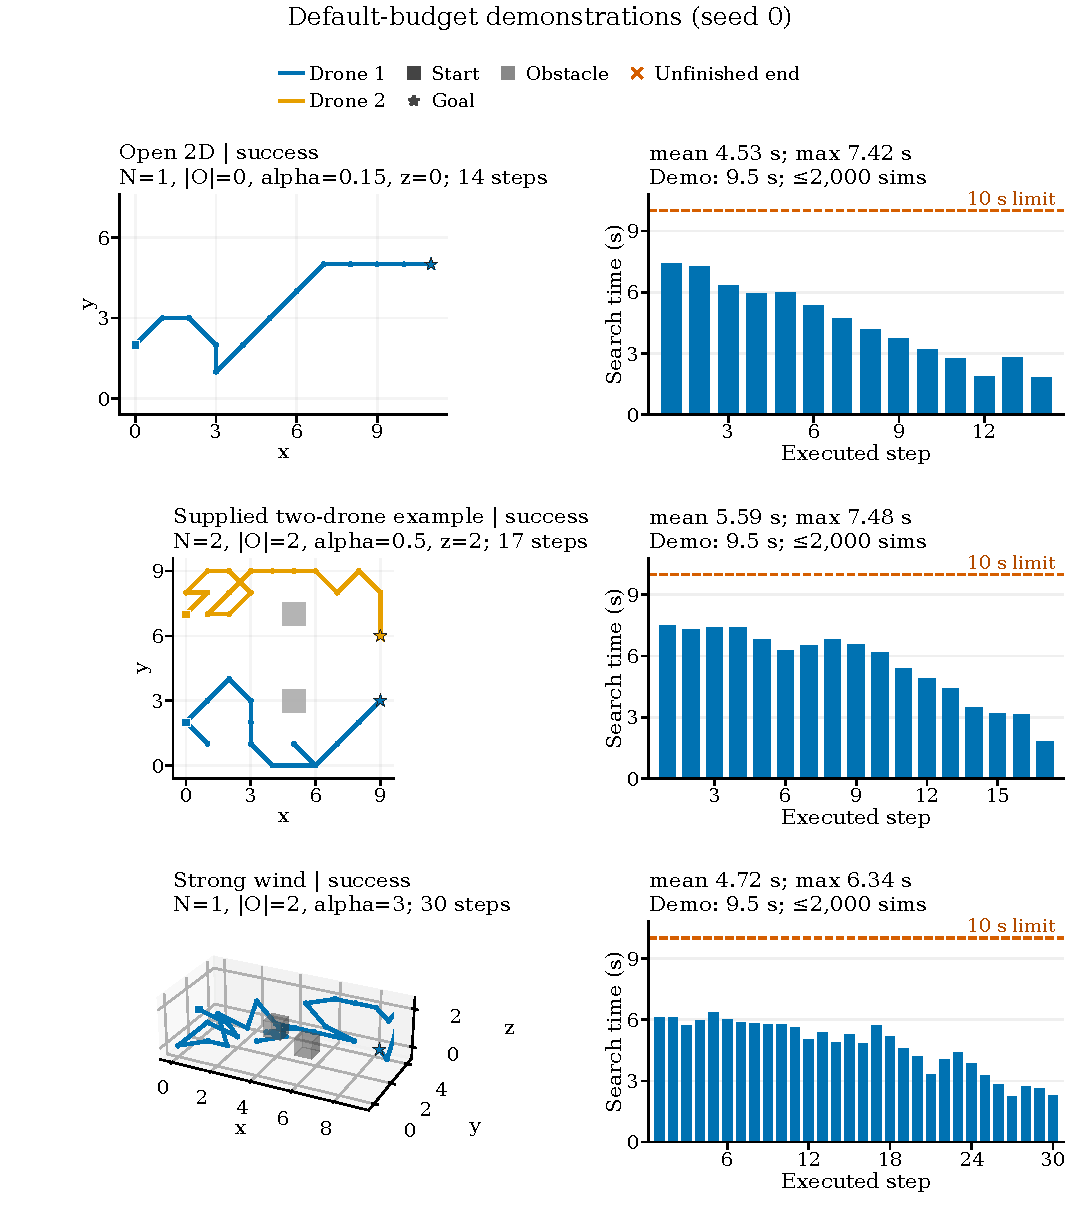
\includegraphics[width=\linewidth]{figures/scenario_examples_1.pdf}
\caption{Default-budget demonstrations: open navigation, the supplied
example, strong wind and four-drone 3D flight.}
\end{figure}

\clearpage
\begin{figure}[H]
\centering
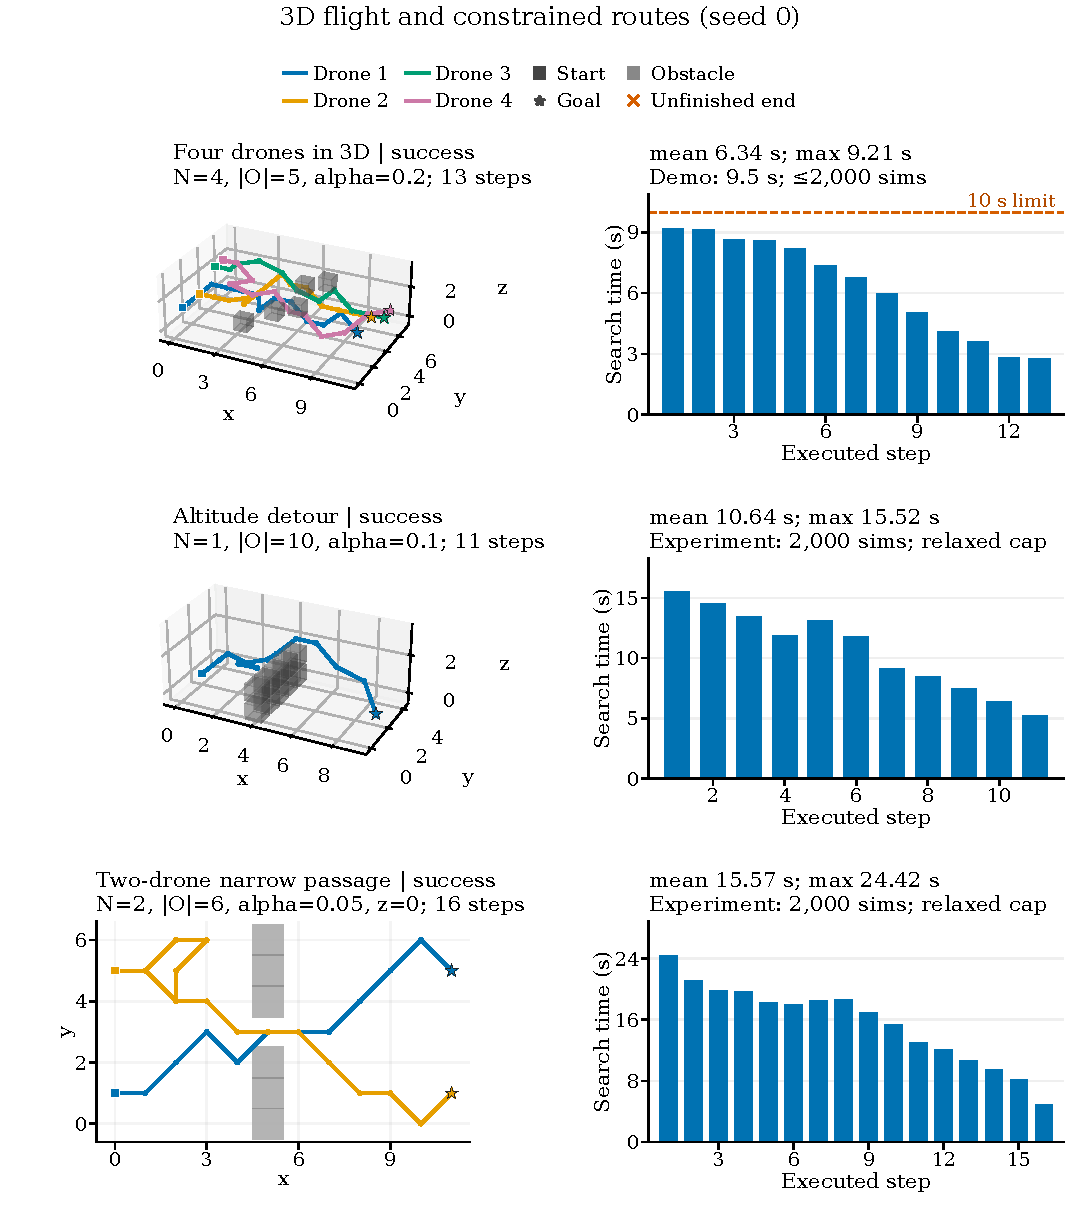
\includegraphics[width=\linewidth]{figures/scenario_examples_2.pdf}
\caption{Fixed-simulation examples: altitude detours, narrow passage,
clutter and a wall gap. The wall-gap layout has seven obstacles.}
\end{figure}

\clearpage
\begin{figure}[H]
\centering
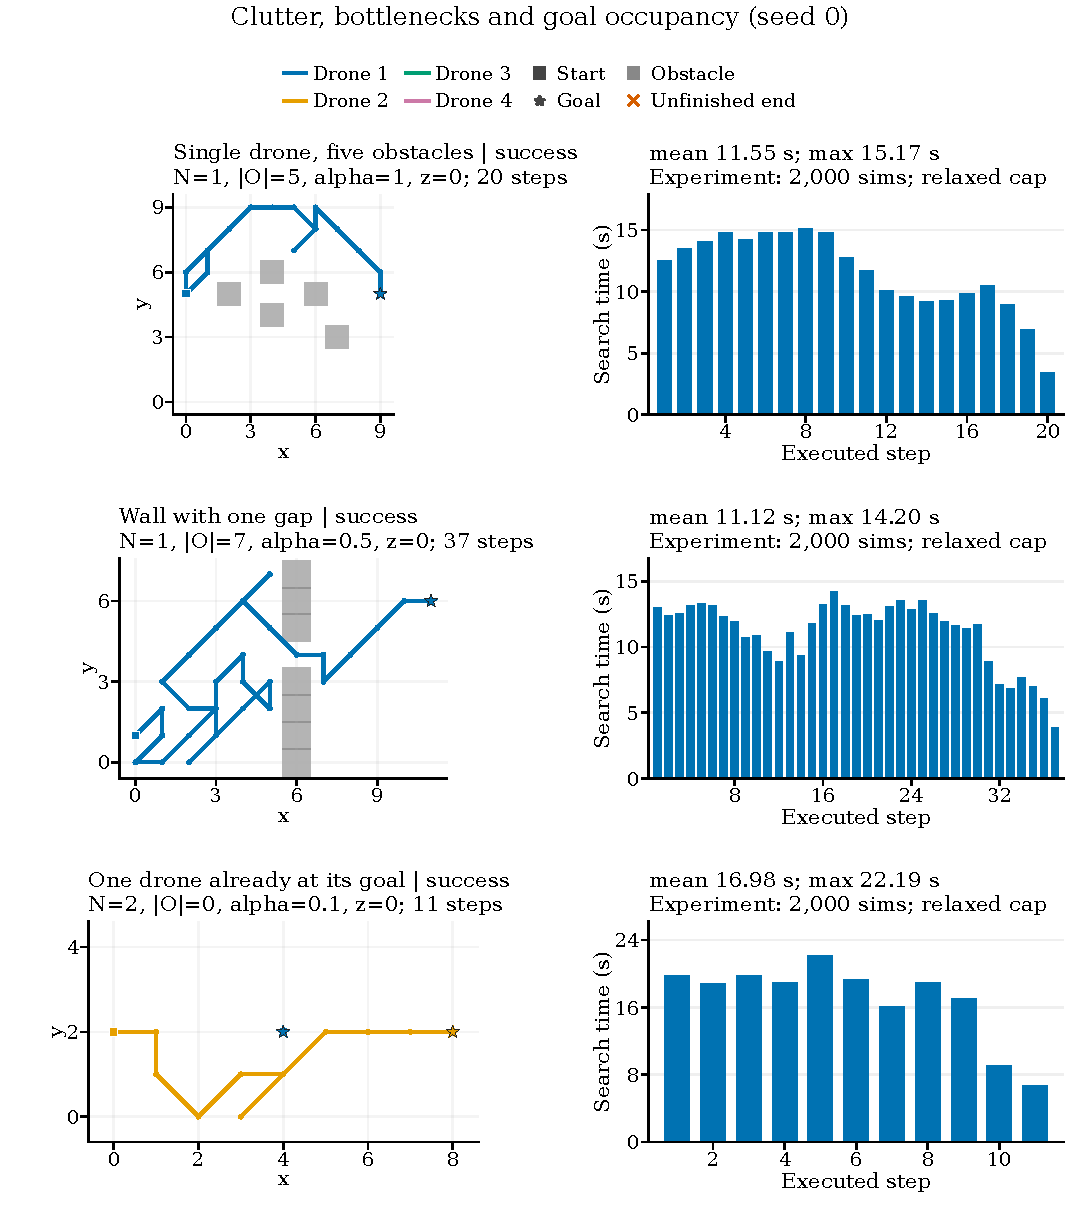
\includegraphics[width=\linewidth]{figures/scenario_examples_3.pdf}
\caption{Fixed-simulation examples: an occupied goal, separate altitude
layers, a shared corridor and a collision. The corridor has eight obstacles.
Timings on this and the preceding sheet are not demo deadline measurements.}
\end{figure}


\end{document}
